\documentclass[a4paper]{article}
\usepackage{geometry}
\geometry{
	a4paper,
	total={170mm,257mm},
	left=27mm,
	right=30mm,
	top=30mm,
	bottom= 30mm
}
\usepackage{tabu}
\usepackage[english]{babel}
\usepackage[utf8]{inputenc}
\usepackage{longtable}
\usepackage{amsmath}
\usepackage{graphicx}
\usepackage{enumitem}
\usepackage[colorinlistoftodos]{todonotes}
\usepackage{tikz}
\newcommand*\circled[1]{\tikz[baseline=(char.base)]{
		\node[shape=circle,draw,inner sep=0.5pt] (char) {#1};}}
\usetikzlibrary{fit,positioning}
\usepackage{authblk}
\usepackage{natbib}
\usepackage[algo2e]{algorithm2e}
\usepackage{algorithmic}  
\usepackage{algorithm}
\usepackage{comment}
\usepackage{array}% http://ctan.org/pkg/array
\makeatletter
\g@addto@macro{\endtabular}{\rowfont{}}% Clear row font
\makeatother
\newcommand{\rowfonttype}{}% Current row font
\newcommand{\rowfont}[1]{% Set current row font
	\gdef\rowfonttype{#1}#1%
}
\newcolumntype{L}{>{\rowfonttype}l}
\title{A Network Model for Continuous Time Textual Communications\\ with Application to Government Email Corpora}
%\author{Bomin Kim}

\author[1]{Bomin Kim}
\author[1]{Zachary Jones}
\author[1]{Bruce Desmarais}
\author[2,3]{Hanna Wallach}
\affil[1]{Pennsylvania State University}
\affil[2]{Microsoft Research NYC}
\affil[3]{University of Massachusetts Amherst}

\begin{document}
\maketitle
\begin{abstract}
	
	\noindent In this paper, we introduce the interaction-partitioned topic model
	(IPTM)---a probabilistic model of who communicates with whom about
	what, and when. Broadly speaking, the IPTM partitions time-stamped
	textual communications, such as emails, according to both the network
	dynamics that they reflect and their content. To do this, it draws on
	the Cox multiplicative intensity model---a generative model for ties
	that tend toward structural features such as reciprocated dyads and
	triangles---and latent Dirichlet allocation---a generative model for
	topic-based content. The IPTM assigns each communication to an
	``interaction pattern," characterized by a set of dynamic network
	features and a distribution over a shared set of topics. We use the
	IPTM to analyze emails sent between department managers in two county
	governments in North Carolina; one of these email corpora covers the
	Outer Banks during the time period surrounding Hurricane Sandy. Via
	this application, we demonstrate that the IPTM is effective at
	predicting and explaining continuous-time textual communications.	
\end{abstract}
\section{Introduction} \label{sec: Introduction}
Since Latent Dirichlet Allocation \citep{Blei2003}, which models of words alone, a variety of useful topic models have been developed by considering additional components other than words. One direction incorporated the network aspect by using the author and receiver information such as Author-Topic Models \citep{rosen2004author}, Author-Recipient-Topic Models and Role-Author-Recipient-Topic Models \citep{mccallum2005topic}, however, all of the models treat the author and recipients as observed variable thus generative processes only involve topics and words in a document. On the other side, there have been a lot of topic
models that focus on the timestamps of documents. For example, Dynamic Topic Models \citep{blei2006dynamic} introduced logistic normal topic models that rely on Markov assumptions with discretization of time, and Topics Over Time \citep{wang2006topics} suggested a countinuous-time model by generating a timestamp from the Beta distribution with its parameter depending on each topic assignment. However none of the above mentioned topic models are jointly dealing with the author-recipient and timestamps of the documents, although it is common in the field of dynamic network analysis to study who connects to whom and when $(i, j, t)$. \\ \newline
In this paper, we develop the interaction-partitioned topic model (IPTM), a dynamic topic model which reflects the network dynamics (sender or author, recipients, and timestamp) and the contents of the document (topics and words). By assigning each communication to an
``interaction pattern," IPTM connects the two separate processes, tie generating process from the Cox multiplicative intensity model and content generating process from latent Dirichlet allocation, and model the process of who communicates with whom about what, and when. 
\section{IPTM Model} \label{sec: IPTM Model}
We first introduce the multiplicative Cox intensity model in the context of tie formation process in a continuous-time textual communication network. We then illustrate the generative process of the model which incorporates the generative process of stochastic actor-oriented models and latent Dirichlet allocation. Lastly, specification of the dynamic network statistics used is demonstrated. For concreteness, we frame our discussion of this model in terms of email data, although it is generally applicable to any similarly-structured communication data.
\subsection{Cox Multiplicative Intensity} \label{subsec: Cox Multiplicative Intensity}
Assume we have a collection of documents, consisting of $D$ number of unique documents. A single email, indexed by $d \in \{1,...,D\}$, is represented by the four components ($i^{(d)}, J^{(d)}, t^{(d)},  W^{(d)}$). The first two are the sender and receiver of the email: an integer $i^{(d)} \in \{1,...,A\}$ indicates the identity of the sender out of $A$ number of actors (or nodes) and an integer vector $J^{(d)} = \{j_r^{(d)}\}_{r=1}^{|J^{(d)}|} $ indicates the identity of the receiver (or receivers) out of $A-1$ number of actors (by excluding self-loop), where $|J^{(d)}|\in \{1,...,A-1\}$ denotes the total number of the receivers. Next, $t^{(d)}$ is the (unix time-based) timestamp of the email $d$, and $W^{(d)} = \{w^{(d)}_m \}_{n=1}^{N^{(d)}}$ is a set of tokens that comprise the text of the email. In this section, we only consider the first three , ($i^{(d)}, J^{(d)}, t^{(d)}$), and explain how we apply multiplicative intensity model to the generating process of a document (or a tie). \\ \newline 
\begin{comment}
Let $T$ denote the survival time. In our context, survival times measure the time to send the document. Following the typical survival analysis framework, the distribution of $T$ is described or characterized by three functions, namely:
\begin{itemize}
	\item [1. ] the probability density function $f(t)$: \newline the probability of sending a document in a small interval per unit time
	\begin{align*}
	f(t) &= \lim\limits_{\Delta t \rightarrow 0+} \frac{P\{\mbox{a document sent in the interval } (t, t+ \Delta t)\}}{\Delta t} \\&
	= \lim\limits_{\Delta t \rightarrow 0+} \frac{P[T \in (t, t+ \Delta t)]}{\Delta t}
	\end{align*}
	\item [2. ] the survival function $S(t)$\newline
	the probability that a document is not sent until time $t$
	\begin{align*}
	S(t) &= P(T>t) \\& = \int_{t}^{\infty} f(u)du \\& = 1-F(t)
	\end{align*}
	\item [3. ] the hazard rate function $\lambda(t)$ \newline
	the probability of sending a document in a very short interval $t$ to  $t+ \Delta t$  per unit time, given that the document has not sent until time $t$ 
		\begin{align*}
		\lambda(t) &= \lim\limits_{\Delta t \rightarrow 0+} \frac{P\{\mbox{a document sent in the interval } (t, t+ \Delta t)|\mbox{not sent until time $t$}\}}{\Delta t} \\&
		= \lim\limits_{\Delta t \rightarrow 0+} \frac{P\{t \leq T < t+ \Delta t|T\geq t\}}{\Delta t}
		\end{align*}
		Since our $T$ is a continuous random variable, we have
				\begin{align*}
				\lambda(t) &=\frac{f(t)}{S(t)} = \frac{f(t)}{1-F(t)} = -\frac{d}{dt} \mbox{log}[S(t)].
				\end{align*}
		The hazard function can alternatively be represented in terms of the cumulative hazard function
			\begin{align*}
			\Lambda(t) &=  \int_{0}^{t} \lambda(u)du = -\mbox{log}[S(t)],
			\end{align*}
			which establishes another relationship
				\begin{align*}
				S(t) &=  \mbox{exp}(-\Lambda(t)).
				\end{align*}
\end{itemize}
Given the equations above, we derive:
				\begin{align*}
				f(t) &=-\frac{d}{dt}S(t) = -\frac{d}{dt}\mbox{exp}(-\Lambda(t)) = \lambda(t)S(t) = \lambda(t)e^{-\int_{0}^{t}\lambda(u)du},
				\end{align*}
and thus following the dominant method for summarizing survival data, we will use the hazard function $\lambda(t)$ for the generative process of the document. Now we move to Cox multiplicative intensity model \citep{cox1992regression} using covariates
that depend on the history of the process. Cox multiplicative intensity model, also known as the Cox proportional hazards (PH) model, is the most common approach to model covariate effects on survival. \\ \newline
\end{comment}
The interaction-partitioned topic model (IPTM) assigns each communication to an ``interaction pattern," characterized by a set of dynamic network features and a distribution over a shared set of topics. Here we illustrate how a set of dynamic network features contribute uniquely identifies each interaction pattern. Assume that each interaction pattern $c \in \{1,...,C\}$ has an $A\times A$ stochastic intensity (or hazard) matrix of $\boldsymbol{\lambda}^{(c)}(t) = \{\{\lambda^{(c)}_{ij}(t)\}_{i=1}^{A}\}_{j=1}^{A}$, where $\lambda^{(c)}_{ij}(t)$=P\{for interaction pattern $c$, $i\rightarrow j$ occurs in time interval $[t, t+dt)$, given that it has not ben sent until time $t$\}. There could be various static and dynamic covariates $\boldsymbol{x}^{(c)}_t(i, j)$ that affects the stochastic intensity, however, we decide to use the covariates
that depend on the history of the process, considering the strong recency and reciprocity effects of textual communications, especially emails. The detailed specifications of the dynamic network covariates are illustrated in Section \ref{subsec: Dynamic covariates}.\\ \newline
Following the multiplicative Cox model, the $(i, j)^{th}$ element of the intensity matrix $\boldsymbol{\lambda}^{(c)}(t)$ forms:
\begin{equation}
\lambda^{(c)}_{ij}(t)=\lambda_0\cdot \mbox{exp}\Big\{\boldsymbol{\beta}^{(c)T}\boldsymbol{x}^{(c)}_t(i, j)\Big\}\cdot 1\{j \in \mathcal{A}_{\backslash i}\},
\end{equation}
where $\lambda_0$ is the common baseline hazards for the overall interaction (assume that $\lambda_0$ does not depend on $t$), $\boldsymbol{\beta}^{(c)}$ is an unknown vector of coefficients in $\boldsymbol{R}^{p}$, $\boldsymbol{x}^{(c)}_t(i, j)$ is a vector of the $p$-dimensional dynamic network statistics for directed edge $(i, j)$ at time $t$, and $\mathcal{A}_{\backslash i}$ is the predictable receiver set of sender $i$ within the set of all possible actors $\mathcal{A}$ (no self-loop). Equivalently, by fixing $\lambda_0=1$, we can avoid unknown baseline hazard rate and rewrite (1) as: 
\begin{equation}
\lambda^{(c)}_{ij}(t)= \mbox{exp}\Big\{\boldsymbol{\beta}^{(c)T}\boldsymbol{x}^{*(c)}_t(i, j)\Big\}\cdot 1\{j \in \mathcal{A}_{\backslash i}\},
\end{equation}
where the first element of $\boldsymbol{\beta}^{(c)}$ corresponds to the deviation from $\lambda_0$, by including the intercept term and setting $\boldsymbol{x}^{*(c)}_t(i, j)=(\boldsymbol{1}, \boldsymbol{x}^{(c)}_t(i, j))$. Since multicast interactions—those involving a single sender but multiple
receivers—are allowed for this model, we expand the rate of interaction between sender $i$ and the receivers in a set $J$ as:
\begin{equation}
\lambda^{(c)}_{iJ}(t)= \mbox{exp}\Big\{\sum\limits_{j \in J} \boldsymbol{\beta}^{(c)T}\boldsymbol{x}^{*(c)}_t(i, j)\Big\}\cdot \prod\limits_{j \in J}1\{j \in \mathcal{A}_{\backslash i}\}.
\end{equation}
In case of single receivers ($|J|=1$),  Equation (3) is reduced to Equation (2), thus in the following sections we use the Equation (3) of multicast cases as a general form of the stochastic intensity between the sender and receivers.
\begin{comment}
Conditioned upon the existence of a unique document at some particular time $t$, the probability that the document is sent from $i$ to $j$ is
	\begin{align*}
	&L_{ij}(\boldsymbol{\beta}^{(c)}) = \frac{\mbox{exp}\Big\{ \boldsymbol{\beta}^{(c)T}\boldsymbol{x}^{*(c)}_t(i, j)\Big\}}{\mbox{exp}\Big\{\sum\limits_{j \in \mathcal{A}_{\backslash i}} \boldsymbol{\beta}^{(c)T}\boldsymbol{x}^{*(c)}_t(i, j)\Big\}},
	\end{align*}
and considering the multicasts and treating the documents being statistically independent, the joint probability, the full likelihood function is:
\begin{equation}
L(\boldsymbol{\beta}^{(c)})=\prod_{d: c^{(d)}=c} \frac{\mbox{exp}\{\sum\limits_{j \in J^{(d)}} \boldsymbol{\beta}^{(c)T}x^{(c)}_{t^{(d)}}(i^{(d)}, j)\}}{\sum\limits_{\substack{J \subseteq \mathcal{A}_{\backslash i^{(d)}} \\|J|=|J^{(d)}|}} \mbox{exp}\{\sum\limits_{j \in J} \boldsymbol{\beta}^{(c)T}x^{(c)}_{t^{(d)}}(i^{(d)}, j)\}}.
\end{equation}
This is exactly the form of the partial likelihood function of \cite{cox1992regression}, however, in our case it is full likelihood since we do not have baseline hazard (incorporated into $\boldsymbol{x}$) in $\lambda^{(c)}_{ij}(t|\boldsymbol{x}_t^{*(c)}(i, j))$. Therefore, for interaction pattern $c=1,...,C$, estimation for $\boldsymbol{\beta}^{(c)}$ proceeds by maximizing the log-likelihood function: 
\begin{equation}
\mbox{log}L(\boldsymbol{\beta}^{(c)})=\sum_{d: c^{(d)}=c} \Big\{\sum\limits_{j \in J^{(d)}} \boldsymbol{\beta}^{(c)T}\boldsymbol{x}^{(c)}_{t^{(d)}}(i^{(d)}, j)\}-\mbox{log}[{\sum\limits_{\substack{J \subseteq \mathcal{A}_{\backslash i^{(d)}} \\|J|=|J^{(d)}|}} \mbox{exp}\{ \boldsymbol{\beta}^{(c)T}\boldsymbol{x}^{(c)}_{t^{(d)}}(i^{(d)}, j)\}}]\Big\},
\end{equation}
where the risk set in the denominater is defined as all possible sets of recievers with the same cardinality as $|J^{(d)}|$. To prevent the bias in the parameter estimates from treating multicast interactions as well as achieve computational efficiency, we use the log-partial likelihood defined in \cite{PerryWolfe2012}:
\begin{equation}
\mbox{log}\widetilde{L}(\boldsymbol{\beta}^{(c)})=\sum_{d: c^{(d)}=c} \Big\{\sum\limits_{j \in J^{(d)}}\boldsymbol{\beta}^{(c)T}\boldsymbol{x}^{(c)}_{t^{(d)}}(i^{(d)}, j)-|J^{(d)}|\mbox{log}\big[\sum_{j\in \mathcal{A}_{\backslash i^{(d)}}}\mbox{exp}\{\boldsymbol{\beta}^{(c)T}\boldsymbol{x}^{(c)}_{t^{(d)}}(i^{(d)}, j)\}\big]\Big\},
\end{equation}
where the approximation $\mbox{log}{L}_t(\boldsymbol{\beta}^{(c)})\approx \mbox{log}\widetilde{L}_t(\boldsymbol{\beta}^{(c)})$ is suggested in \cite{PerryWolfe2012} by replacing the sum over all sets of size $|J^{(d)}|$ in (5) with a sum over all multisets of size $|J^{(d)}|$ (i.e. allowing duplicate elements from $\mathcal{A}_{\backslash i^{(d)}}$) as below: 
\begin{equation}
\begin{split}
\mbox{log}[{\sum\limits_{\substack{J \subseteq \mathcal{A}_{\backslash i^{(d)}} \\|J|=|J^{(d)}|}} \mbox{exp}\{\sum\limits_{j \in J} \boldsymbol{\beta}^{(c)T}\boldsymbol{x}^{(c)}_{t^{(d)}}(i^{(d)}, j)\}}]&\approx
\mbox{log}[({\sum\limits_{j \in \mathcal{A}_{\backslash i^{(d)}} } \mbox{exp}\{\boldsymbol{\beta}^{(c)T}\boldsymbol{x}^{(c)}_{t^{(d)}}(i^{(d)}, j)\}})^{|J^{(d)}|}]\\& = |J^{(d)}|\times\mbox{log}\big[\sum_{j\in \mathcal{A}_{\backslash i^{(d)}}}\mbox{exp}\{\boldsymbol{\beta}^{(c)T}\boldsymbol{x}^{(c)}_{t^{(d)}}(i^{(d)}, j)\}\big]
\end{split}
\end{equation}
\end{comment}
\subsection{Generative Process} \label{subsec: Generative Process}
The interaction-partitioned topic model (IPTM) is a probabilistic model of who communicates with whom about what, and when. The generative process of IPTM consists of two parts: 1) generation of the ties (i.e. `who', `whom', and `when') and 2) generation of content (i.e. `what'). The tie generating process resembles that of stochastic actor-oriented models (SAOMs) of \cite{snijders1996stochastic}, and the content generating process directly follows latent Dirichlet allocation (LDA) of \cite{Blei2003}. In this section, we illustrate the two generative process separately, and show how the two processes can jointly generate a document.
\subsubsection{Tie Generating Process}\label{subsubsec: Tie Generating Process}
Motivated from stochastic actor-oriented model (SAOM) of \cite{snijders2017stochastic}, a model which assumes that the network evolves as a stochastic process `driven by the actors’, we assume the following generative process for each document $d$ in a corpus $D$:
\begin{itemize}
	\item[1.] Choose the interaction pattern $c^{(d)} \sim \mbox{Multinomial}(\gamma)$
	\item[2.] (Data augmentation) For each sender $i \in \{1,...,A\}$, create a list of receivers $J_i$ by applying the Bernoulli probabilities to every $j \in \mathcal{A}_{\backslash i}$
	\begin{align*} I(i \rightarrow j) \sim \mbox{Ber}\Big(1-\mbox{exp}(-\delta\lambda^{(c^{(d)})}_{ij}(t_+^{(d-1)}))\Big),
	\end{align*}
	where the probability is called a Bernoulli-Poisson (BerPo) link function \citep{zhou2015infinite} and $\delta$ is a tuning parameter to control the number of multicasts. Note that $_+$ denotes including the timepoint itself, meaning that $\lambda_{ij}$ is obtained using the history of interactions until and including $t^{(d-1)}$. (i.e. $\lambda^{(c^{(d)})}_{ij}(t_+^{(d-1)})=\mbox{exp}\Big\{\boldsymbol{\beta}^{(c^{(d)})T}\boldsymbol{x}^{*(c^{(d)})}_{t^{(d-1)}_+}(i, j)\Big\}\cdot 1\{j \in \mathcal{A}_{\backslash i}\}$)
	\item[3.] For each sender $i = 1,...,A$, generate the time increments $\Delta T_{i{J_i}} \sim \mbox{Exp}(\lambda_{i{J_i}}(t_+^{(d-1)}))$, where $\lambda_{i{J_i}}(t_+^{(d-1)})= \mbox{exp}\Big\{\sum\limits_{j \in{J_i}}\boldsymbol{\beta}^{(c^{(d)})T}\boldsymbol{x}^{*(c^{(d)})}_{t^{(d-1)}_+}(i, j)\Big\}\cdot \prod\limits_{j \in J_i}1\{j \in \mathcal{A}_{\backslash i}\}$
	 \item[4.] Set the timestamp $t^{(d)} = t^{(d-1)}+\mbox{min}(\Delta T_{i{J_i}})$, $i^{(d)} = i_{\mbox{min}(\Delta T_{i{J_i}})}$, and $J^{(d)} = J_{i^{(d)}}$.
\end{itemize}
\subsubsection{Content Generating Process} \label{subsubsec: Content Generating Process}
The content generating process is a simple addition of the interaction pattern assignment to the existing generative process of Latent Dirichlet Allocation \cite{Blei2003}. This concept is also very similar to the Cluster-Based Topic Modelling \citep{wallach2008structured}, in a way that every document is assigned its group $c^{(d)}$ and then each document-specific topic distribution $\boldsymbol{\theta}^{(d)}$ can instead be drawn from a group-specific $\mbox{Dir}(\alpha^{(c^{(d)})}, \boldsymbol{m}^{(c^{(d)})})$, thereby respecting the document groupings. We assume the following generative process for each document $d$ in a corpus $D$:
\begin{itemize}
	\item[1.] Choose the interaction pattern $c^{(d)} \sim \mbox{Multinomial}(\gamma)$
	\item[2.] Choose the number of words $N^{(d)} \sim \mbox{Poisson}(\zeta)$
	\item[3.] Choose document-topic distribution $\boldsymbol{\theta}^{(d)}\sim \mbox{Dir}(\alpha^{(c^{(d)})}, \boldsymbol{m}^{(c^{(d)})})$
	\item[4.] For each of the $N^{(d)}$ words $w_n^{(d)}$:
 		\begin{itemize}
 			\item[(a)] Choose a topic $z_n^{(d)} \sim \mbox{Multinomial}(\boldsymbol{\theta}^{(d)})$
 			\item[(b)] Choose a word $w_n^{(d)} \sim\mbox{Multinomial} (\phi^{(z_n^{(d)})})$
 		\end{itemize}
\end{itemize}
\subsubsection{Joint Generative Process of Document} \label{subsubsec: Joint Generative Process of Document}
 Below are the joint generative process for each document in a corpus $D$ and the corresponding plate notation (Figure 1).
\begin{itemize}
	\item[1.] {$\boldsymbol{\phi}^{(k)} \sim \mbox{Dir}(\beta, \bf u)$} \textbf{[See Algorithm 1]}\\
	- A “topic” $k$ is characterized by a discrete distribution over $V$ word types with probability vector $\phi^{(k)}$. A symmetric Dirichlet prior $\bf u$ with the concentration parameter $\beta$ is placed.
	\item[2.] For the interaction pattern $c=1,...,C$,  \textbf{[See Algorithm 2]}: 
		\begin{itemize}
			\item [(a)] $\boldsymbol{\beta}^{(c)}\sim \mbox{Normal}(\textbf{0}, \sigma^2I_P)$ \\
			- The vector of coefficients depends on the interaction pattern $c$. This means that there is variation in the degree of influence from the dynamic network statistics.
			\item [(b)]  Set $\alpha^{(c)}$ and $\boldsymbol{m}^{(c)}$\\
			- The topic proportions for documents in the same cluster share the same parameters in the Dirichlet distribution. How we choose these parameters will be explained in Section \ref{subsec: Asymmetric Dirichlet prior over theta}.
		\end{itemize}
	\item[3.] For the document $d=1,...,D$ \textbf{[See Algorithm 3]}:
	\begin{itemize}
				\item[(a)] $c^{(d)}\sim \mbox{Multinomial}(\boldsymbol{\gamma})$\\
				- Each document $d$ is associated with one ``interaction pattern" among $C$ different types, with the parameter $\boldsymbol{\gamma}$. Here, we assign the prior for the multinomial parameter $\boldsymbol{\gamma} \sim \mbox{Dir}({\eta}, \boldsymbol{l})$, where $\boldsymbol{l}$ is a symmetric base prior by default.
				\item[(b)]  $N^{(d)} \sim \mbox{Poisson}(\zeta)$\\
				- The number of words in the document is chosen from Poisson distribution, and $\zeta$ can be either fixed or estimated.
				\item[(c)] Calculate $\boldsymbol{x}^{*(c^{(d)})}_{t_+^{(d-1)}}(i, j)$ and the corresponding $\boldsymbol{\lambda}^{(c^{(d)})}(t)$\\
			- The dynamic network statistics are calculated based on the documents of the same interaction pattern, using the history of interactions until (and including) the last document.
		\item[(d)] Choose $t^{(d)}$, $i^{(d)}$, and $J^{(d)}$ following Section 1.2.1. (i.e. $\mathbf{N}^{(d|c^{(d)})}(t^{(d)}) \sim \mbox{CP}(\boldsymbol{\lambda}^{(c^{(d)})}(t_+^{(d-1)})))$\\
		- $\mathbf{N}^{(d|c^{(d)})}(t^{(d)})$ is a $A\times A$ matrix where $(i^{(d)}, j)^{th}$ ($j \in J^{(d)}$) elements are 1 and the rest are 0.
		\item[(e)] $\boldsymbol{\theta}^{(d)}\sim \mbox{Dir}(\alpha^{(c^{(d)})}, \boldsymbol{m}^{(c^{(d)})})$\\
		- Each email has a discrete distribution over topics $\boldsymbol{\theta}^{(d)}$, and the topic proportions for documents in the same cluster share the same parameters in the Dirichlet distribution.
	\item[(f)] For each of the word $n = 1,...,N^{(d)}$:
\begin{itemize}
	\item [(f1)] $z_n^{(d)} \sim \mbox{Multinomial}(\boldsymbol{\theta}^{(d)})$
	\item [(f2)] $w_n^{(d)} \sim\mbox{Multinomial} (\phi^{(z_n^{(d)})})$
\end{itemize} 
	\end{itemize}
\end{itemize}
\begin{algorithm}[H]
	\SetAlgoLined
	\caption{Topic Word Distributions}
	\For{k=1 to K}{
		draw $\boldsymbol{\phi}^{(k)}$ $\sim$ Dir($\beta, \bf u$)
	}
\end{algorithm}
\begin{algorithm}[H]
	\SetAlgoLined
	\caption{Interaction Pattern-unique Parameters}
	\For{c=1 to C}{
draw $\boldsymbol{\beta}^{(c)}\sim \mbox{Normal}(\textbf{0}, \sigma^2I_P)$\\
set $\alpha^{(c)}$ and $\boldsymbol{m}^{(c)}$
	}
\end{algorithm}
	\begin{algorithm}[H]
		\SetAlgoLined
		\caption{Document Generating Process}
		\For{d=1 to D}{
			draw $c^{(d)}$ $\sim$ Multinomial($\boldsymbol{\gamma}$)\\
			draw $N^{(d)} \sim \mbox{Poisson}(\zeta)$\\
			draw ($t^{(d)}, i^{(d)}, J^{(d)})$ using $\mathbf{N}^{(d|c^{(d)})}(t^{(d)}) \sim \mbox{CP}(\boldsymbol{\lambda}^{(c^{(d)})}( t_+^{(d-1)}))$\\
			draw $\boldsymbol{\theta}^{(d)}\sim \mbox{Dir}(\alpha^{(c^{(d)})}, \boldsymbol{m}^{(c^{(d)})})$\\
				\For{n=1 to ${N}^{(d)}$}{
					draw $z_n^{(d)} \sim \mbox{Multinomial}(\boldsymbol{\theta}^{(d)})$\\
					{draw $w_n^{(d)} \sim\mbox{Multinomial} (\boldsymbol{\phi}^{(z_n^{(d)})})$
					}}
		}
	\end{algorithm}
 \small
 \begin{figure}[ht]
 	\centering
\scalebox{0.74}{  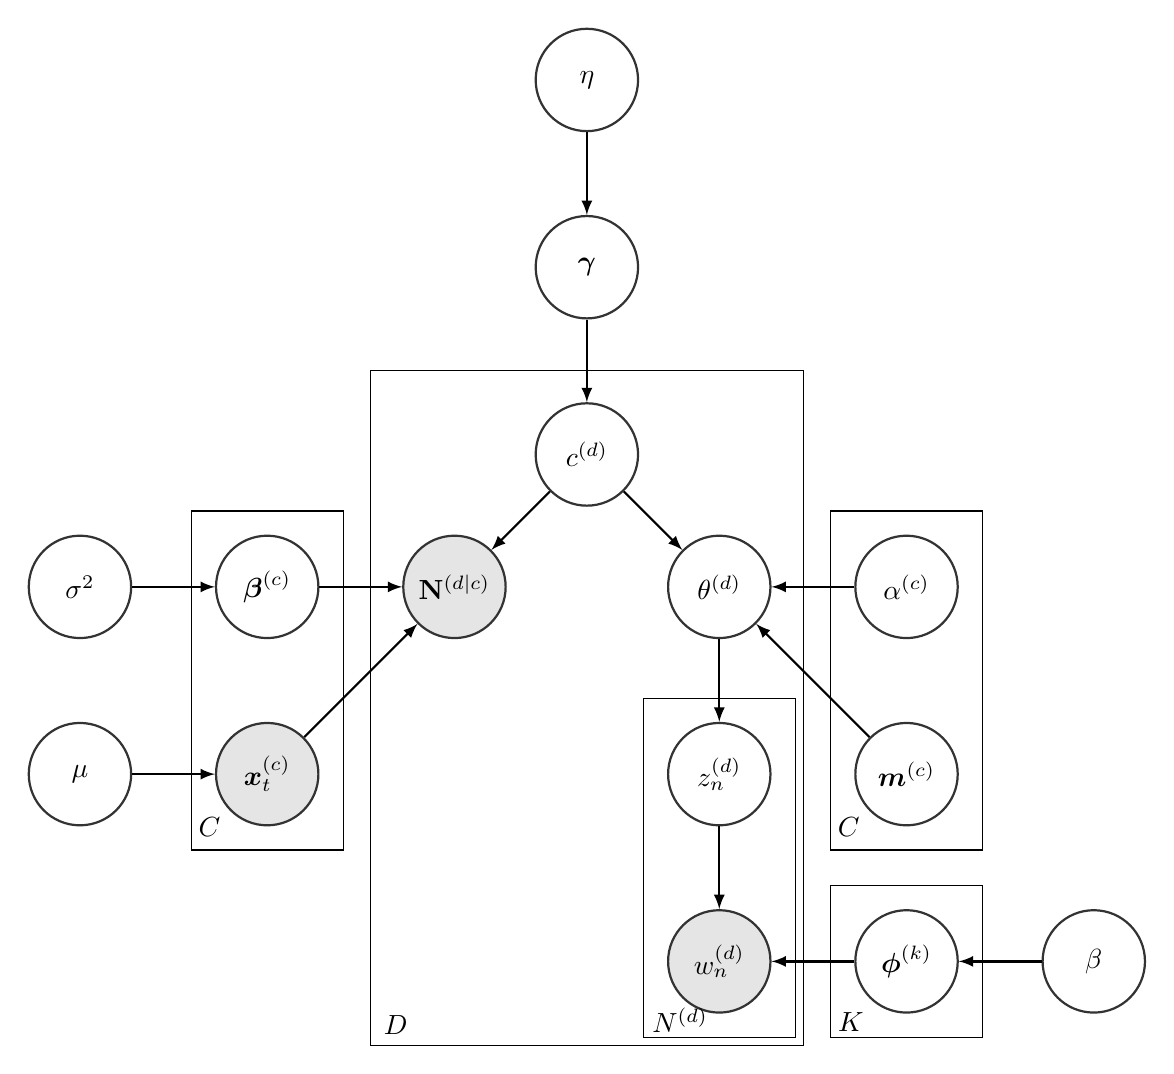
\begin{tikzpicture}
 		\tikzstyle{main}=[circle, minimum size = 13mm, thick, draw =black!80, node distance = 10.5mm]
 		\tikzstyle{connect}=[-latex, thick]
 		\tikzstyle{box}=[rectangle, draw=black!100]
 		\node[main, fill = white!100] (gamma) [label=center:$\boldsymbol{\gamma}$] { };
 		\node[main] (c) [below=of gamma,label=center:$c^{(d)}$] { };
 			\node[main] (eta) [above=of gamma,label=center:${\eta}$] { };
 			\node[main, fill = black!10] (N) [below left=of c ,label=center:$\mathbf{N}^{(d|c)}$] { };	
 				\node[main] (theta) [below right=of c,label=center:${\theta}^{(d)}$] { };
 					\node[main] (z) [below=of theta,label=center:$z_n^{(d)}$] {};
 						\node[main, fill = black!10] (w) [below=of z,label=center:$w_n^{(d)}$] { };
 								\node[main] (phi) [right=of w,label=center:$\boldsymbol{\phi}^{(k)}$] { };
 								\node[main] (beta2) [right=of phi, label=center:$\beta$] { };
 									\node[main] (beta) [left=of N ,label=center:$\boldsymbol{\beta}^{(c)}$] { };
 									\node[main, fill = black!10] (x) [below=of beta ,label=center:$\boldsymbol{x}^{(c)}_t$] { };
 										\node[main] (sigma) [left=of beta,label=center:$\sigma^2$] { };
 										\node[main] (mu) [left=of x,label=center:$\mu$] { };
 											\node[main] (alpha) [right=of theta,label=center:${\alpha}^{(c)}$] { };
 											\node[main] (m) [below=of alpha,label=center:$\boldsymbol{m}^{(c)}$] { };
 											
  		\path (gamma) edge [connect] (c)
  			(c) edge [connect] (N)
  				(c) edge [connect] (theta)
  					(theta) edge [connect] (z)
  						(z) edge [connect] (w)
  							(phi) edge [connect] (w)
  								(beta2) edge [connect] (phi)
  									(x) edge [connect] (N)
  									(beta) edge [connect] (N)
  									(mu) edge [connect] (x)
  									(sigma) edge [connect] (beta)
  										(alpha) edge [connect] (theta)
  										(m) edge [connect] (theta)
  			(eta) edge [connect] (gamma);
  				\node[rectangle, inner sep=4mm, draw=black!100, fit =(c) (z) (w) (N) ] {};
  				\node[rectangle, inner sep=2mm, fit= (c) (N) ,label=below left:$D$, xshift=4mm, yshift=-44.5mm] {};
  				\node[rectangle, inner sep=3mm, draw=black!100, fit= (phi)] {};
  					\node[rectangle, inner sep=0mm, fit= (phi),label=below left:$K$, xshift=2.5mm, yshift=1.5mm] {};
  						\node[rectangle, inner sep=0mm, fit= (w),label=below left:$N^{(d)}$, xshift=6.5mm, yshift=2mm] {};
  							\node[rectangle, inner sep=3mm,draw=black!100, fit= (w)(z)] {};
  								\node[rectangle, inner sep=3mm,draw=black!100, fit= (beta)(x)] {};
  								\node[rectangle, inner sep=4mm, fit= (beta)(x) ,label= below left:$C$, xshift=6mm, yshift=-5.5mm] {};
  										\node[rectangle, inner sep=3mm,draw=black!100, fit= (alpha)(m)] {};
  										\node[rectangle, inner sep=4mm, fit= (alpha)(m) ,label= below left:$C$, xshift=6mm, yshift=-5.5mm] {};
 	 		\end{tikzpicture}}
 	\caption{Plate notation of IPTM}
 	\label{fig:plate}
 \end{figure}
\iffalse
 \small
 \begin{figure}[ht]
 	\centering
 	\scalebox{0.9}{ 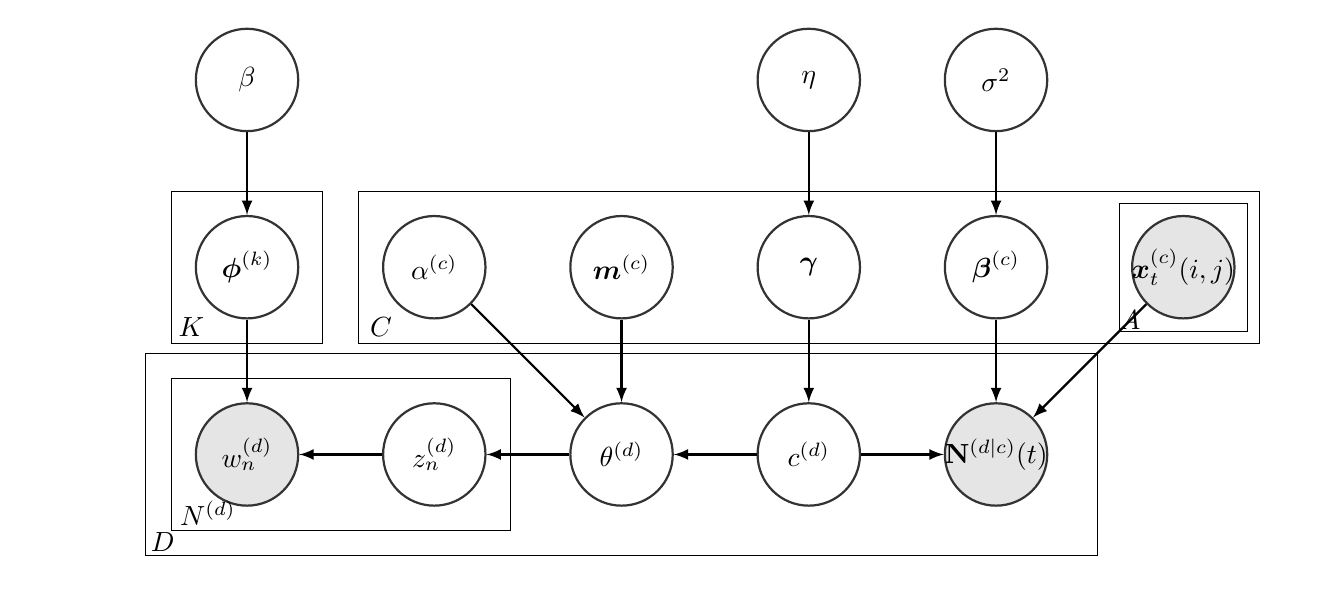
\begin{tikzpicture}
 		\tikzstyle{main}=[circle, minimum size = 13mm, thick, draw =black!80, node distance = 10.5mm]
 		\tikzstyle{connect}=[-latex, thick]
 		\tikzstyle{box}=[rectangle, draw=black!100]
 		\node[main, fill = white!100] (gamma) [label=center:$\boldsymbol{\gamma}$] { };
 		\node[main] (c) [below=of gamma,label=center:$c^{(d)}$] { };
 		\node[main, fill = black!10] (N) [right=of c ,label=center:$\mathbf{N}^{(d|c)}(t)$] { };	
 		\node[main] (eta) [above=of gamma,label=center:${\eta}$] { };
 		\node[main] (beta) [above=of N ,label=center:$\boldsymbol{\beta}^{(c)}$] { };
 		\node[main, fill = black!10] (x) [right=of beta ,label=center:$\boldsymbol{x}^{(c)}_t{(i,j)}$] { };
 		\node[main] (theta) [left=of c,label=center:${\theta}^{(d)}$] { };
 		\node[main] (sigma) [above=of beta,label=center:$\sigma^2$] { };
 		\node[main] (z) [left=of theta,label=center:$z_n^{(d)}$] {};
 		\node[main, fill = black!10] (w) [left=of z,label=center:$w_n^{(d)}$] { };
 		\node[main] (phi) [above=of w,label=center:$\boldsymbol{\phi}^{(k)}$] { };
 		\node[main] (beta2) [above=of phi, label=center:$\beta$] { };
 		\node[main] (alpha) [above=of z,label=center:${\alpha}^{(c)}$] { };
 		\node[main] (m) [above=of theta,label=center:$\boldsymbol{m}^{(c)}$] { };
 		\path (gamma) edge [connect] (c)
 		(z) edge [connect] (w)
 		(theta) edge [connect] (z)
 		(phi) edge [connect] (w)
 		(beta2) edge [connect] (phi)
 		(sigma) edge [connect] (beta)
 		(x) edge [connect] (N)
 		(beta) edge [connect] (N)
 		(c) edge [connect] (N)
 		(c) edge [connect] (theta)
 		(alpha) edge [connect] (theta)
 		(m) edge [connect] (theta)
 		(eta) edge [connect] (gamma);
 		\node[rectangle, inner sep=2.5mm, fit=  (x),label=below left:$A$, xshift=5mm, yshift=5mm] {};
 		\node[rectangle, inner sep=3mm,draw=black!100, fit= (beta)(alpha) (m)(x)] {};
 		\node[rectangle, inner sep=4mm, fit= (beta)(alpha) (m)(x) ,label= below left:$C$, xshift=-41mm, yshift=5.5mm] {};
 		\node[rectangle, inner sep=3mm, draw=black!100, fit= (phi)] {};
 		\node[rectangle, inner sep=1.5mm, draw=black!100, fit= (x) ] {};
 		\node[rectangle, inner sep=0mm, fit= (phi),label=below left:$K$, xshift=2.5mm, yshift=1.5mm] {};
 		\node[rectangle, inner sep=0mm, fit= (w),label=below left:$N^{(d)}$, xshift=6.5mm, yshift=2mm] {};
 		\node[rectangle, inner sep=3mm,draw=black!100, fit= (w)(z)] {};
 		\node[rectangle, inner sep=3.5mm, fit= (c) (N) ,label=below left:$D$, xshift=-81mm, yshift=1.5mm] {};
 		\node[rectangle, inner sep=6.2mm, draw=black!100, fit =(c) (z) (w) (N) ] {};
 		\end{tikzpicture}}
 	\caption{Plate notation of IPTM}
 	\label{fig:plate1}
 \end{figure}
\fi
 \subsection{Dynamic covariates to measure network effects} \label{subsec: Dynamic covariates}
 The network statistics $\boldsymbol{x}^{*(c)}_t(i, j)$ of Equation (2), corresponding to the ordered pair $(i, j)$, can be time-invariant (such as gender) or time-dependent (such as the number of two-paths from $i$ to $j$ just before time $t$). Since time-invariant covariates can be easily specified in various manners (e.g. homophily or group-level effects), here we only consider specification of dynamic covariates.\\
 \begin{figure}[ht]
 	\centering
 	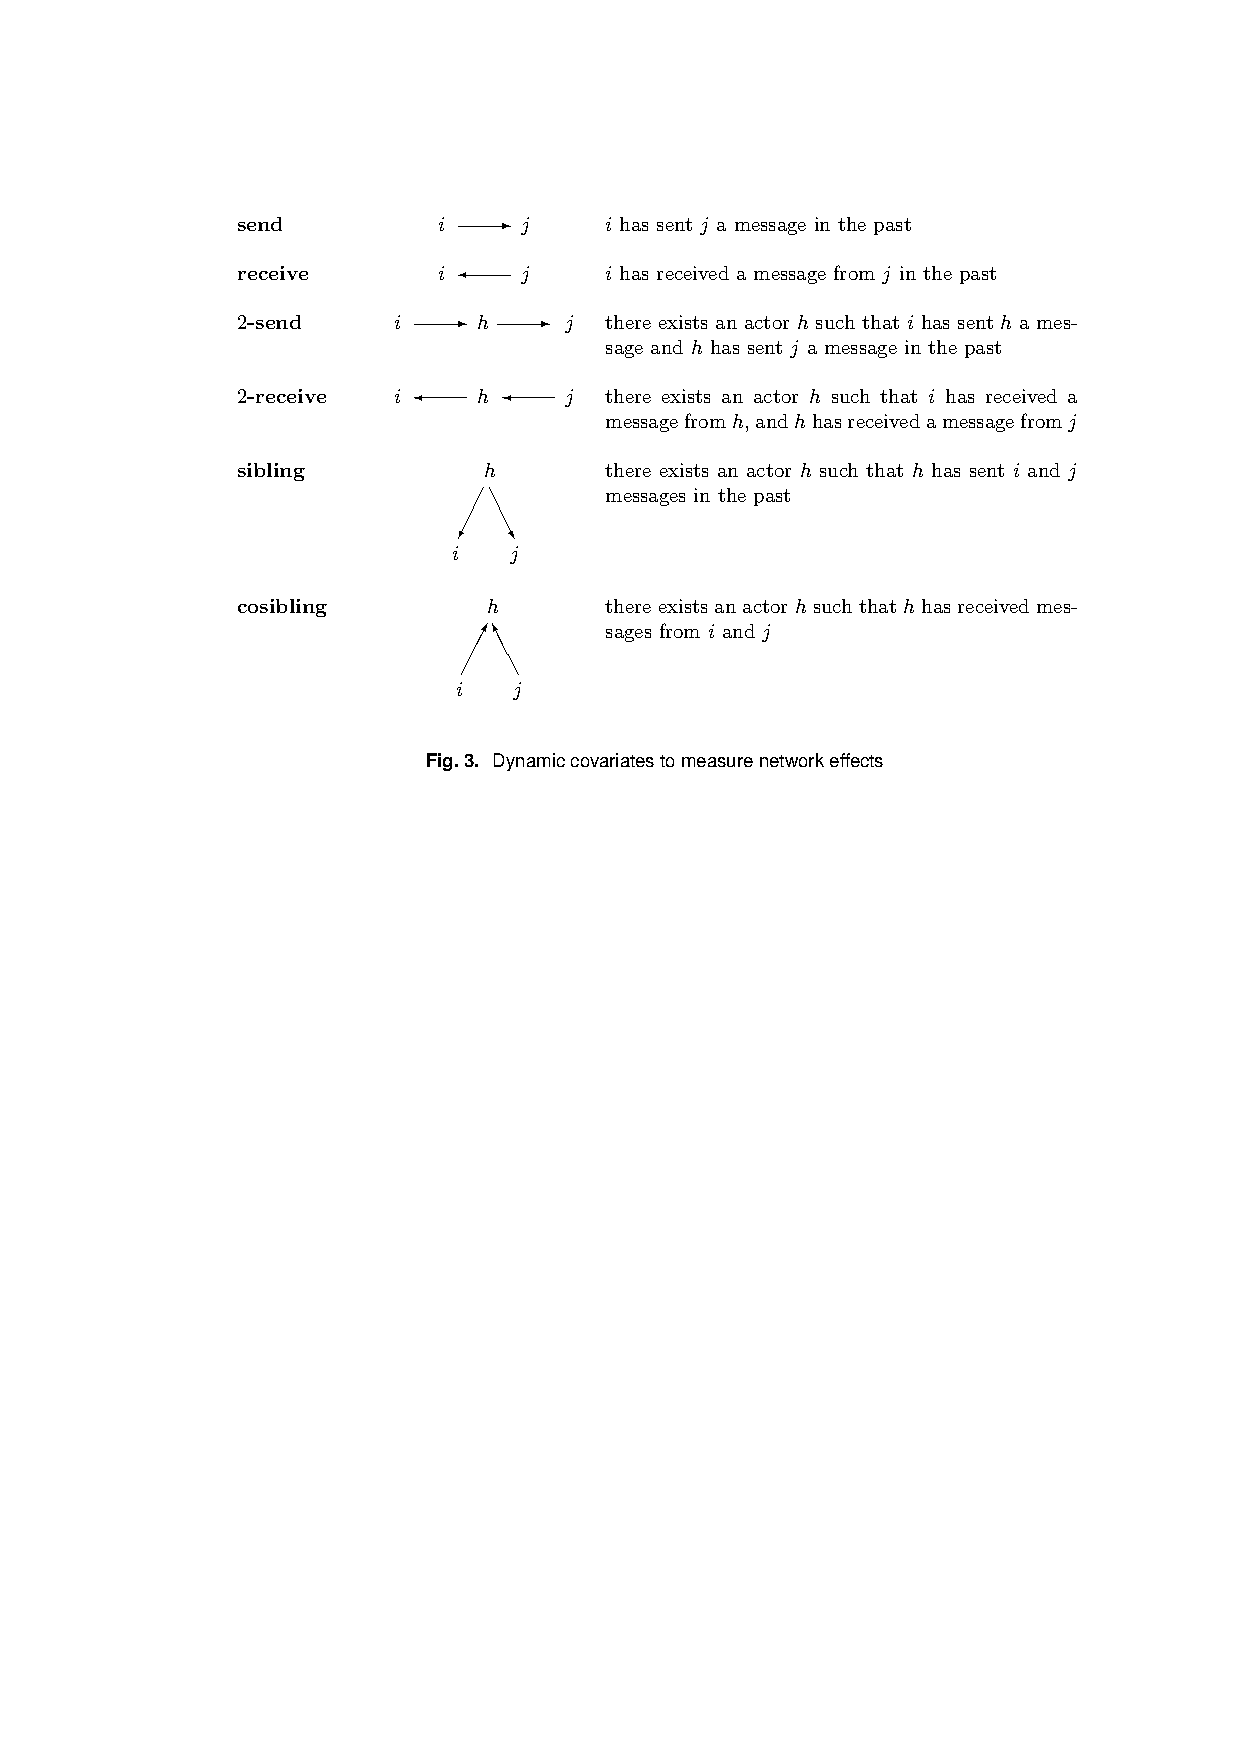
\includegraphics[width=0.56\textwidth]{PerryWolfe.pdf} 
 	\label{fig:PerryWolfeplot}
 \end{figure}
 \newline Following \cite{PerryWolfe2012} (refer to Fig.3 of \cite{PerryWolfe2012} attached above), we use 4 effects as components of $\boldsymbol{x}^{*(c)}_t(i, j)$, including the intercept to estimate the baseline intensities. The two behaviors (send and receive) are dyadic, involving exactly two actors,
 while the one is triadic (sum of 2-send, 2-receive, sibling, and cosibling), involving exactly three actors. In addition to the ones from \cite{PerryWolfe2012}, we also include the indegree for receiver and outdegree for sender effects to measure the popularity and centrality. However, one different point from the existing specification is that we define the effects not to be based on finite sub-interval, which require large number of dimension. Instead, we create a single statistic for each effect by incorporating the recency of event into the statistic itself. As a result, all of the statistics can be seen as time-weighted dynamic network statistics.
 \begin{itemize}[leftmargin=*,rightmargin=-1cm]
 	\item [1.] $\mbox{intercept}^{(c)}_t(i, j) = 1$
 	\item [2.]  $\mbox{send}^{(c)}_t(i, j)=\sum\limits_{d: c^{(d)}=c}\sum\limits_{d: t^{(d)}<t} I\{i\rightarrow j\}\cdot g(t-t^{(d)})$
 	\item [3.] $\mbox{receive}^{(c)}_t(i, j)=\sum\limits_{d: c^{(d)}=c}\sum\limits_{d: t^{(d)}<t} I\{j\rightarrow i\}\cdot g(t-t^{(d)})$
 	\item [4.] $\mbox{triangle}^{(c)}_t(i, j)=\sum\limits_{d: c^{(d)}=c}\sum\limits_{h \neq i, j}\Big(\sum\limits_{d: t^{(d)}<t}  I\{i\rightarrow h \mbox{ or } h\rightarrow j \}\cdot g(t-t^{(d)})\Big)\Big(\sum\limits_{d: t^{(d)}<t} I\{j\rightarrow h \mbox{ or } h\rightarrow j\}\cdot g(t-t^{(d)})\Big)$
 	\item [5.]  $\mbox{outdegree}^{(c)}_t(i)=\sum\limits_{d: c^{(d)}=c}\sum\limits_{j\neq i}\sum\limits_{d: t^{(d)}<t} I\{i\rightarrow j\}\cdot g(t-t^{(d)})$
 	\item [6.] $\mbox{indegree}^{(c)}_t(j)=\sum\limits_{d: c^{(d)}=c}\sum\limits_{i \neq j}\sum\limits_{d: t^{(d)}<t} I\{j\rightarrow i\}\cdot g(t-t^{(d)})$
 \end{itemize}
\vspace{3mm}
Here, time decaying function $g(t-t^{(d)})$ reflects the difference between current time $t$ and the timestamp of previous email $t^{(d)}$, thus measuring the recency. Inspired by the self-exciting Hawkes process, which is often used to model the temporal effect of email data, we can take the exponential kernel $g(t-t^{(d)})=e^{-\mu(t-t^{(d)})}$ where $\mu$ is the parameter of speed at which sender replies to emails, with larger values indicating faster response times. Indeed, $\mu^{-1}$ is the expected number of hours it takes to reply to a typical email. For simplicity, in our simulation we fixed $\mu=0.05$ (i.e. $g(t-t^{(d)})=e^{-0.05(t-t^{(d)})}$), but $\mu$ can also be esitimated.
  \section{Inference} \label{sec: Inference}
In this case, what we actually observe are the tokens $\mathcal{W}=\{\boldsymbol{w}^{(d)} \}_{d=1}^{D}$ and the sender, recipient, and timestamps $(i=i^{(d)}, j=J^{(d)}, t=t^{(d)})$ of the email in the form of the counting process $\mathcal{N}=\{\boldsymbol{N}^{(d)}(t^{(d)}) \}_{d=1}^{D}.$ Next,  $\mathcal{X}=\{\boldsymbol{x}^{(c)}_{t^{(d)}}(i, j)\}_{d=1}^{D}$ is the metadata, and the latent variables are $\Phi=\{\boldsymbol{\phi}^{(k)}\}_{k=1}^{K}, \Theta=\{\boldsymbol{\theta}^{(d)} \}_{d=1}^{D}, \mathcal{Z}=\{\boldsymbol{z}^{(d)} \}_{d=1}^{D}, \mathcal{C}=\{{c}^{(d)} \}_{d=1}^{D},$ and $\mathcal{B}=\{\boldsymbol{\beta}^{(c)} \}_{c=1}^{C}$.\\
 \newline 
 Below is the the big joint distribution
 \begin{equation}
 \begin{aligned}
 & P(\Phi, \Theta, \mathcal{W}, \mathcal{Z}, \mathcal{C}, \mathcal{B}, \mathcal{N}| \mathcal{X}, \beta, \boldsymbol{u}, \alpha, \boldsymbol{m}, \boldsymbol{\gamma}, \boldsymbol{\eta}, \sigma^2) \\& 
 =  P(\mathcal{W}, \mathcal{Z}, \mathcal{C}, \mathcal{B}, \mathcal{N}| \Phi, \Theta, \mathcal{X}, \boldsymbol{\gamma}, \boldsymbol{\eta}, \sigma^2) P(\Phi, \Theta |\beta, \boldsymbol{u}, \alpha, \boldsymbol{m})
 \\&= P( \mathcal{W}| \mathcal{Z}, \Phi)P(\mathcal{Z}|\Theta)P(\mathcal{N}|\mathcal{C}, \mathcal{X}, \mathcal{B})P(\mathcal{B}|\mathcal{C}, \sigma^2)P(\Phi|\beta, \boldsymbol{u})P(\Theta|\mathcal{C}, \alpha, \boldsymbol{m})P(\mathcal{C}|\boldsymbol{\gamma})P(\boldsymbol{\gamma}|\boldsymbol{\eta})
 \end{aligned}
 \end{equation}
 Now we can integrate out $\Phi$ and $\Theta$ in latent Dirichlet allocation by applying Dirichlet-multinomial conjugacy. See APPENDIX B for the detailed steps. After integration, we obtain below:
 \begin{equation}
 \propto P(\mathcal{W}|\mathcal{Z})P( \mathcal{Z}|\mathcal{C}, \beta, \boldsymbol{u}, \alpha, \boldsymbol{m})P(\mathcal{N}|\mathcal{C}, \mathcal{B}, \mathcal{X})P(\mathcal{B}|\mathcal{C}, \sigma^2)P(\mathcal{C}|\boldsymbol{\gamma})
 \end{equation}
 Then, we only have to perform inference over the remaining unobserved latent variables $\mathcal{Z}, \mathcal{C},$ and $\mathcal{B}$, using the equation below:
 \begin{equation}
 P( \mathcal{Z}, \mathcal{C}, \mathcal{B}|\mathcal{W}, \mathcal{N}, \mathcal{X}, \beta, \boldsymbol{u}, \alpha, \boldsymbol{m}, \boldsymbol{\gamma}, \boldsymbol{\eta}, \sigma^2) \propto P(\mathcal{W},  \mathcal{Z}, \mathcal{C}, \mathcal{B}, \mathcal{N} | \mathcal{X}, \beta, \boldsymbol{u}, \alpha, \boldsymbol{m}, \boldsymbol{\gamma}, \boldsymbol{\eta}, \sigma^2)
 \end{equation}
 Either Gibbs sampling or Metropolis-Hastings algorithm is applied by sequentially resampling each latent variables from their respective conditional posterior.
  \subsection{Data augmentation} \label{subsec: Data augmentation}
  As mentioned earlier in Section \ref{subsubsec: Tie Generating Process}, we use data augmentation to make inference on $\mathcal{B}=\{\boldsymbol{\beta}^{(c)} \}_{c=1}^{C}$. That is, for every document $d$, we generate the latent sender-receivers $(i, J_i)$ for all $i \in \mathcal{A}_{\backslash i}$ and plug the generated sets into the likelihood function of $\boldsymbol{\beta}^{(c)}$. Note that in latent data generating step, the sets $(i, J_i)$ should account for the probability $P(\mbox{latent receiver}| \mbox{latent time} < \mbox{observed time})$. This probability can be derived fairly easily using Bayes' theorem: \\\newline
Let $t^{(d)}$ be the observed time, $t_i$ be the latent time associated with the latent email sent by $i$, and $i \rightarrow j$ be an indicator of whether sender $i$ added $j$ to the latent email receivers (i.e. $j \in J_i$). 
  \begin{equation}
  \begin{split}
P(i \rightarrow j|\Delta T_{i{J_i}} > \Delta T_{i^{(d)}{J^{(d)}}}) &= \frac{P(\Delta T_{i{J_i}} > \Delta T_{i^{(d)}{J^{(d)}}}|i \rightarrow j)P(i \rightarrow j)}{P(\Delta T_{i{J_i}} > t^{(d)})}  \\&= \frac{P(\Delta T_{i{J_i}}> \Delta T_{i^{(d)}{J^{(d)}}}|i \rightarrow j)P(i \rightarrow j)}{P(\Delta T_{i{J_i}} > \Delta T_{i^{(d)}{J^{(d)}}}|i \rightarrow j)P(i \rightarrow j) + P(\Delta T_{i{J_i}} > \Delta T_{i^{(d)}{J^{(d)}}}|i \not\to j)P(i \not\to j)} 
  \end{split}
  \end{equation}
  where $P(\Delta T_{i{J_i}}> \Delta T_{i^{(d)}{J^{(d)}}}|i \rightarrow j)$ and $P(\Delta T_{i{J_i}} >\Delta T_{i^{(d)}{J^{(d)}}}|i \not\to j)$ are given by the cumulative exponential distributions associated with the respective $\lambda_{iJ_i}(t_+^{(d-1)})$ and $P(i \rightarrow j)$ and $P(i \not\to j)$ are given by the Bernoulli transformation in Section \ref{subsubsec: Tie Generating Process}. Therefore, we determine the latent ties $I(i\rightarrow j)$ from Bernoulli distribution of probability:
    \begin{equation}
 \frac{e^{-(t^{(d)}-t^{(d-1)})\lambda^j_{iJ_i}(t_+^{(d-1)})}(1-e^{-\delta\lambda^{(c^{(d)})}_{ij}(t_+^{(d-1)})})}{e^{-(t^{(d)}-t^{(d-1)})\lambda^j_{iJ_i}(t_+^{(d-1)})}(1-e^{-\delta\lambda^{(c^{(d)})}_{ij}(t_+^{(d-1)})})+e^{-(t^{(d)}-t^{(d-1)})\lambda^{-j}_{iJ_i}(t_+^{(d-1)})}(e^{-\delta\lambda^{(c^{(d)})}_{ij}(t_+^{(d-1)})})},
    \end{equation}
    \textcolor{red}{QUESTION: We need baseline $\lambda_{iJ_i}$ before we add $j$ into the recipient set.....}\\
    where $\lambda^j_{iJ_i}$ is calculated from the receiver set of $i$ that includes $j$, while $\lambda^{-j}_{iJ_i}$ is calculated from the receiver set of $i$ that excludes $j$.\\ \newline
Next, when it comes to the inference, conditioned upon the existence of the $d^{th}$ document at some particular time $t^{(d)}$, the probability that the document is sent from $i^{(d)}$ to $J^{(d)} (=J_{i^{(d)}})$ is
  \begin{equation}
  \begin{split}
  \mathcal{L}(\boldsymbol{\beta}^{(c^{(d)})}) &= P\Big(\Delta T_{i^{(d)}{J^{(d)}}}\sim\mbox{Exp}(\lambda_{i^{(d)}{J^{(d)}}}(t_+^{(d-1)}))\Big)\times P\Big(\mbox{min}(\Delta T_{i{J_i}}) = \Delta T_{i^{(d)}{J^{(d)}}}\Big)\times P\Big(\mbox{Edge creations}\Big)\\&
  =\Big(\lambda_{i^{(d)}{J^{(d)}}}(t_+^{(d-1)})e^{-(t^{(d)}-t^{(d-1)})\lambda_{i^{(d)}{J^{(d)}}}(t_+^{(d-1)})}\Big)\times \Big(e^{-(t^{(d)}-t^{(d-1)})\sum\limits_{i \neq i^{(d)}}\lambda_{i{J_i}}(t_+^{(d-1)})}\Big)\\ & \quad\quad\times \Big(\prod_{i\in \mathcal{A}}\prod_{j \in \mathcal{A}_{\backslash i }} (1-e^{-\delta\lambda_{ij}(t_+^{(d-1)})})^{I(j \in J_i)}(e^{-\delta\lambda_{ij}(t_+^{(d-1)})})^{1-I(j \in J_i)}\Big)\\
  & = \Big(\lambda_{i^{(d)}{J^{(d)}}}(t_+^{(d-1)})e^{-(t^{(d)}-t^{(d-1)})\sum\limits_{i \in \mathcal{A}}\lambda_{i{J_i}}(t_+^{(d-1)})}\Big) \times \Big(\prod_{i\in \mathcal{A}}\prod_{j \in \mathcal{A}_{\backslash i }} (e^{\delta\lambda_{ij}(t_+^{(d-1)})}-1)^{I(j \in J_i)}e^{-\delta\lambda_{ij}(t_+^{(d-1)})}\Big),
  \end{split}
  \end{equation}
  Applying this to the every document in the corpus and taking the log,  we obtain the full likelihood function used for the inference of $\{\boldsymbol{\beta}^{(c)}\}_{c=1}^C$ as:
  \begin{equation}
  \begin{split}
  \ell(\boldsymbol{\beta}^{(c^{(d)})}) &=\sum_{d=1}^D\Big\{\sum\limits_{j \in{J_{i^{(d)}}}}\boldsymbol{\beta}^{(c^{(d)})T}\boldsymbol{x}^{*(c^{(d)})}_{t^{(d-1)}_+}(i^{(d)}, j)-(t^{(d)}-t^{(d-1)})\sum\limits_{i \in \mathcal{A}}e^{\sum\limits_{j \in{J_i}}\boldsymbol{\beta}^{(c^{(d)})T}\boldsymbol{x}^{*(c^{(d)})}_{t^{(d-1)}_+}(i, j)}\\&\quad\quad+\sum\limits_{i\in \mathcal{A}}\sum\limits_{j \in \mathcal{A}_{\backslash i }}\Big(I(j \in J_i)\cdot\mbox{log}(e^{\delta e^{\boldsymbol{\beta}^{(c^{(d)})T}\boldsymbol{x}^{*(c^{(d)})}_{t^{(d-1)}_+}(i, j)}}-1)-\delta e^{\boldsymbol{\beta}^{(c^{(d)})T}\boldsymbol{x}^{*(c^{(d)})}_{t^{(d-1)}_+}(i, j)}\Big)\Big\},
  \end{split}\end{equation}
  and since Equation (10) above is the joint likelihood function of the sender, receivers and timestamp $(i^{(d)}, J^{(d)}, t^{(d)})$, it will be used for $P( \mathbf{N}^{(d)}{(t^{(d)})}| c^{(d)}=c, \mathcal{C}_{\backslash d}, \mathcal{B}, \mathcal{N}_{\backslash d}, \mathcal{X})$ in the next following steps.
  \newpage
 \subsection{Resampling $\mathcal{C}$} \label{subsec: Resampling C}
 The first variable we are going to resample is the document-interaction pattern assignments, one document at a time. To obtain the Gibbs sampling equation, which is the posterior conditional probability for the interaction pattern $\mathcal{C}$ for $d^{th}$ document, i.e. $P(c^{(d)}=c|\mathcal{W}, \mathcal{Z},  \mathcal{C}_{\backslash d}, \mathcal{B}, \mathcal{N}, \mathcal{X}, \beta, \boldsymbol{u}, \alpha, \boldsymbol{m}, \boldsymbol{\gamma}, \boldsymbol{\eta}, \sigma^2)$. We can derive the equation as below:
 \begin{equation}
 \begin{aligned} & P(c^{(d)}=c|\mathcal{W}, \mathcal{Z}, \mathcal{C}_{\backslash d}, \mathcal{B}, \mathcal{N}, \mathcal{X}, \beta, \boldsymbol{u}, \alpha, \boldsymbol{m}, \boldsymbol{\gamma}, \boldsymbol{\eta}, \sigma^2)\\
 &\propto P(c^{(d)}=c, \boldsymbol{w}^{(d)}, \boldsymbol{z}^{(d)},  \mathbf{N}^{(d)}{(t^{(d)})}|\mathcal{W}_{\backslash d}, \mathcal{Z}_{\backslash d},\mathcal{C}_{\backslash d}, \mathcal{B}, \mathcal{N}_{\backslash d}, \mathcal{X}, \beta, \boldsymbol{u}, \alpha, \boldsymbol{m}, \boldsymbol{\gamma}, \boldsymbol{\eta}, \sigma^2)\\& \propto P(c^{(d)}=c|\mathcal{C}_{\backslash d}, \boldsymbol{\gamma}) P( \mathbf{N}^{(d)}{(t^{(d)})}| c^{(d)}=c, \mathcal{C}_{\backslash d}, \mathcal{B}, \mathcal{N}_{\backslash d}, \mathcal{X})P(\boldsymbol{w}^{(d)}, \boldsymbol{z}^{(d)}|c^{(d)}=c, \mathcal{W}_{\backslash d}, \mathcal{Z}_{\backslash d}, \mathcal{C}_{\backslash d}, \beta, \boldsymbol{u}, \alpha, \boldsymbol{m}), 
 \end{aligned}
 \end{equation}
 where $P(c^{(d)}=c|\mathcal{C}_{\backslash d}, \boldsymbol{\gamma})$ comes from the multinomial prior $\gamma$ and $P( \mathbf{N}^{(d)}{(t^{(d)})}| c^{(d)}=c, \mathcal{C}_{\backslash d}, \mathcal{B}, \mathcal{N}_{\backslash d}, \mathcal{X})$ is the probability of observing a document with the sender, receiver, and time equal to $(i=i^{(d)}, j=J^{(d)}, t=t^{(d)})$, respectively, given a set of parameter values. We will replace this by the partial likelihood in Equation (4) (without the product term since resampling of $c$ is document-specific). For the last term $P(\boldsymbol{w}^{(d)}, \boldsymbol{z}^{(d)}|c^{(d)}=c, \mathcal{W}_{\backslash d}, \mathcal{Z}_{\backslash d}, \mathcal{C}_{\backslash d}, \beta, \boldsymbol{u}, \alpha, \boldsymbol{m})$, we will follow typical LDA approach. \\ \newline Using Bayes' theorem (See APPENDIX C for conditional probabilty of the last term), we have
 \begin{equation}
 \begin{aligned} &=\Big[ \gamma_{c}\Big]\times\Big[ \Big(\lambda_{i^{(d)}{J^{(d)}}}(t_+^{(d-1)})e^{-(t^{(d)}-t^{(d-1)})\sum\limits_{i \in \mathcal{A}}\lambda_{i{J_i}}(t_+^{(d-1)})}\Big) \times \Big(\prod_{i\in \mathcal{A}}\prod_{j \in \mathcal{A}_{\backslash i }} (e^{\delta\lambda_{ij}(t_+^{(d-1)})}-1)^{I(j \in J_i)}e^{-\delta\lambda_{ij}(t_+^{(d-1)})}\Big)\Big]\\&\quad\quad\quad\quad\quad\quad\quad\quad\quad\quad\quad\quad\quad\quad\quad\quad\quad\quad\quad\quad\quad\quad\quad\quad\quad\quad\quad\quad\quad\quad\times\Big[\prod_{n=1}^{N^{(d)}}
 \frac{N_{z_n^{(d)}|d, \backslash d, n}+\alpha^{(c)} \boldsymbol{m}^{(c)}_{z_n^{(d)}}}{N_{\cdot|d, \backslash d, n}+\alpha^{(c)}}\Big],
 \end{aligned}
 \end{equation}
 where $N_{k|d}$ is the number of times topic $k$ shows up in the document $d$. Furthermore, we can take the log of Equation (10) to avoid numerical issue from exponentiation and increase the speed of computation, which becomes:
 \begin{equation}
 \begin{split}
 \Big[\mbox{log}(\gamma_{c})\Big]&+\Big[\sum\limits_{j \in{J_{i^{(d)}}}}\boldsymbol{\beta}^{(c^{(d)})T}\boldsymbol{x}^{*(c^{(d)})}_{t^{(d-1)}_+}(i^{(d)}, j)-(t^{(d)}-t^{(d-1)})\sum\limits_{i \in \mathcal{A}}e^{\sum\limits_{j \in{J_i}}\boldsymbol{\beta}^{(c^{(d)})T}\boldsymbol{x}^{*(c^{(d)})}_{t^{(d-1)}_+}(i, j)}\\&+\sum\limits_{i\in \mathcal{A}}\sum\limits_{j \in \mathcal{A}_{\backslash i }}\Big(I(j \in J_i)\cdot\mbox{log}(e^{\delta e^{\boldsymbol{\beta}^{(c^{(d)})T}\boldsymbol{x}^{*(c^{(d)})}_{t^{(d-1)}_+}(i, j)}}-1)-\delta e^{\boldsymbol{\beta}^{(c^{(d)})T}\boldsymbol{x}^{*(c^{(d)})}_{t^{(d-1)}_+}(i, j)}\Big)\Big]\\&+\Big[\sum_{n=1}^{N^{(d)}}\mbox{log}\Big(N_{z_n^{(d)}|d, \backslash d, n}+\alpha^{(c)} \boldsymbol{m}^{(c)}_{z_n^{(d)}}\Big)-\mbox{log}{\Big(N_{\cdot|d, \backslash d, n}+\alpha^{(c)}}\Big)\Big].
 \end{split}
 \end{equation}
 \subsection{Resampling $\mathcal{Z}$}  \label{subsec: Resampling Z}
 Next, the new values of $z^{(d)}_m$ are sampled for all of the token topic assignments (one token at a time), using the conditional posterior probability of being topic $k$ as we derived in APPENDIX C:
 \begin{equation}
 \begin{aligned} & 
 P(z^{(d)}_n=k|\mathcal{W}, \mathcal{Z}_{\backslash d, n},  \mathcal{C}, \mathcal{B}, \mathcal{N}, \mathcal{X}, \beta, \boldsymbol{u}, \alpha, \boldsymbol{m}, \boldsymbol{\gamma}, \boldsymbol{\eta}, \sigma^2)\\
 & \propto P(z^{(d)}_n=k, w^{(d)}_n|\mathcal{W}_{\backslash d, n}, \mathcal{Z}_{\backslash d,m}, C, \beta, \boldsymbol{u}, \alpha, \boldsymbol{m})
 \end{aligned}
 \end{equation}
 where the subscript $``{\backslash d, n}"$ denotes the exclsuion of position $n$ in $d^{th}$ email. In the last line of equation (13), it is the contribution of LDA, so we can write the conditional probability:
 \begin{equation}
 \begin{aligned} 
 & \propto(N_{k|d, \backslash d, n}+\alpha^{(c^{(d)})} \boldsymbol{m}^{(c^{(d)})}_k)\times\frac{N_{w_n^{(d)}k, \backslash d, n}^{WK}+\beta u_w}{\sum_{w=1}^WN_{wk,  \backslash d, n}^{WK}+\beta}.
 \end{aligned}
 \end{equation}
 which is the well-known form of collapsed Gibbs sampling equation for LDA. After taking the log, we finally obtain:
  \begin{equation}
\mbox{log}(N_{k|d, \backslash d, n}+\alpha^{(c^{(d)})} \boldsymbol{m}^{(c^{(d)})}_k)+\mbox{log}(N_{w_n^{(d)}k, \backslash d, n}^{WK}+\beta u_w)-\mbox{log}({\sum_{w=1}^WN_{wk,  \backslash d, n}^{WK}+\beta}).
  \end{equation}
 \subsection{Resampling $\mathcal{B}$}  \label{subsec: Resampling B}
 Finally, we wan to update the interaction pattern parameter $\boldsymbol{\beta}^{(c)}$, one interaction pattern at a time. For this, we will use the Metropolis-Hastings algorithm with a proposal density $Q$ being the multivariate Gaussian distribution, with variance $\boldsymbol{\beta}^2_B$ (proposal distirbution variance parameters set by the
 user), centered on the current values of $\boldsymbol{\beta}^{(c)}$. Then we draw a proposal $\boldsymbol{\beta}'^{(c)}$ at each iteration. Under symmetric proposal distribution (such as multivariate Gaussian), we cancel out Q-ratio and obtain the acceptance probability equal to:
 \begin{equation}
 \begin{split}
 & \mbox{Acceptance Probability}=
 \begin{cases}  \frac{P(\mathcal{B'}|\mathcal{W}, \mathcal{Z}, \mathcal{C}, \mathcal{N}, \mathcal{X})}{P(\mathcal{B}|\mathcal{W}, \mathcal{Z}, \mathcal{C}, \mathcal{N}, \mathcal{X})}\quad\text{if}  <1\\
 1 \quad \text{else}
 \end{cases}
 \end{split}
 \end{equation}
 After factorization, we get
 \begin{equation}
 \begin{aligned}
 \frac{P(\mathcal{B'}|\mathcal{W},\mathcal{Z}, \mathcal{C}, \mathcal{N}, \mathcal{X})}{P(\mathcal{B}|\mathcal{W}, \mathcal{Z}, \mathcal{C}, \mathcal{N}, \mathcal{X})} &=\frac{P(\mathcal{N}|\mathcal{B'}, \mathcal{W}, \mathcal{Z}, \mathcal{C}, \mathcal{X})P(\mathcal{B'})}{P(\mathcal{N}|\mathcal{B}, \mathcal{W}, \mathcal{Z},  \mathcal{C}, \mathcal{X})P(\mathcal{B})}\\&=\frac{P(\mathcal{N}|\mathcal{C}, \mathcal{X}, \mathcal{B'})P(\mathcal{B'})}{P(\mathcal{N}|\mathcal{C}, \mathcal{X}, \mathcal{B})P(\mathcal{B})},
 \end{aligned}
 \end{equation}
 where $P(\mathcal{N}|\mathcal{C}, \mathcal{X}, \mathcal{B})$ is the partial likelihood in Equation (4).\\ \newline For $P(\mathcal{B})$, we select a multivarate Gaussian priors as mentioned earlier. Similar to what we did in Section \ref{subsec: Resampling C}, we can take the log and obtain the log of acceptance ratio as following:
 \begin{equation}
 \begin{aligned} 
 &\mbox{log}\Big(\phi_d(\boldsymbol{\beta}^{\prime(c)};\mathbf{0}, \sigma^2I_P)\Big)-\mbox{log}\Big(\phi_d(\boldsymbol{\beta}^{(c)};\mathbf{0}, \sigma^2I_P)\Big)\\&+\sum_{d:c^{(d)}=c}\Big[\sum\limits_{j \in{J_{i^{(d)}}}}\boldsymbol{\beta}^{\prime(c^{(d)})T}\boldsymbol{x}^{*(c^{(d)})}_{t^{(d-1)}_+}(i^{(d)}, j)-(t^{(d)}-t^{(d-1)})\sum\limits_{i \in \mathcal{A}}e^{\sum\limits_{j \in{J_i}}\boldsymbol{\beta}^{\prime(c^{(d)})T}\boldsymbol{x}^{*(c^{(d)})}_{t^{(d-1)}_+}(i, j)}\\&+\sum\limits_{i\in \mathcal{A}}\sum\limits_{j \in \mathcal{A}_{\backslash i }}\Big(I(j \in J_i)\cdot\mbox{log}(e^{\delta e^{\boldsymbol{\beta}^{\prime(c^{(d)})T}\boldsymbol{x}^{*(c^{(d)})}_{t^{(d-1)}_+}(i, j)}}-1)-\delta e^{\boldsymbol{\beta}^{\prime(c^{(d)})T}\boldsymbol{x}^{*(c^{(d)})}_{t^{(d-1)}_+}(i, j)}\Big)\Big]\\&-\sum_{d:c^{(d)}=c} \Big[\sum\limits_{j \in{J_{i^{(d)}}}}\boldsymbol{\beta}^{(c^{(d)})T}\boldsymbol{x}^{*(c^{(d)})}_{t^{(d-1)}_+}(i^{(d)}, j)-(t^{(d)}-t^{(d-1)})\sum\limits_{i \in \mathcal{A}}e^{\sum\limits_{j \in{J_i}}\boldsymbol{\beta}^{(c^{(d)})T}\boldsymbol{x}^{*(c^{(d)})}_{t^{(d-1)}_+}(i, j)}\\&+\sum\limits_{i\in \mathcal{A}}\sum\limits_{j \in \mathcal{A}_{\backslash i }}\Big(I(j \in J_i)\cdot\mbox{log}(e^{\delta e^{\boldsymbol{\beta}^{(c^{(d)})T}\boldsymbol{x}^{*(c^{(d)})}_{t^{(d-1)}_+}(i, j)}}-1)-\delta e^{\boldsymbol{\beta}^{(c^{(d)})T}\boldsymbol{x}^{*(c^{(d)})}_{t^{(d-1)}_+}(i, j)}\Big)\Big],
 \end{aligned}
 \end{equation}
 where $\phi_d(\cdot;\mu, \Sigma)$ is the $d$-dimensional multivariate normal density.
 Then the log of acceptance ratio we have is:
 \begin{equation}
 \mbox{log(Acceptance Probability) = min((18), 0) }
 \end{equation}
 To determine whether we accept the proposed update or not, we take the usual approach, by comparing the log of acceptance ratio we have to the log of a sample from uniform(0,1).\\
 \subsection{Asymmetric Dirichlet prior over $\Theta$}  \label{subsec: Asymmetric Dirichlet prior over theta}
 \cite{wallach2009rethinking} demonstrated that the typical implementations of topic models using symmetric Dirichlet priors with fixed concentration parameters often result in less practical results, and the model fitting can be improved by applying an asymmetric Dirichlet prior over the document–topic distributions (i.e. $\Theta$). Therefore, we assign an asymmetric Dirichlet prior over the interaction pattern-topic distributions, $\Theta=\{\boldsymbol{\theta}^{(d)} \}_{d=1}^{D}$, where $\boldsymbol{\theta}^{(d)}$ is drawn from Dir($\alpha^{(c^{(d)})}, \boldsymbol{m}^{(c^{(d)})}$). While \cite{wallach2009rethinking} illustrates two different methods, adding a hierarchy to $\Theta$ and optimizing the hyperparameters ($\alpha$ and $\boldsymbol{m}$), we choose to use hyperparameter
 optimization steps since it is computationally efficient and also sufficient to achieve the desired performance gains. Now, we assume $\boldsymbol{m}^{(c)}$ to be non-uniform base measures (while $\alpha^{(c)}$ is still a fixed concentration parameter), and implement the hyperparameter optimization technique called ``new fixed-point iterations using the Digamma recurrence relation'' in \cite{wallach2008structured} based on Minka’s fixed-point iteration \citep{minka2000estimating}.\\ \newline
 Here we summarize Chapter 2 of \cite{wallach2008structured} and its extension to our IPTM, to illustrate the basic steps and equations used for our optimization. Basically, we want to find the optimal hyperparameter $[\alpha\boldsymbol{m}]^*$ given the data $\mathcal{D}$ such that the probability of the
 data given the hyperparameters $P(\mathcal{D}|\alpha\boldsymbol{m})$ is maximized at $[\alpha\boldsymbol{m}]^*$. After incorporating the interaction pattern component, the evidence is now given by 
 \begin{equation}
 P(\mathcal{D}^{(c)}|\alpha^{(c)}\boldsymbol{m}^{(c)})=\prod_{d:c^{(d)}=c} \frac{\Gamma(\alpha^{(c)})}{\Gamma(N_{\cdot|d}+\alpha^{(c)})}\prod_{k=1}^{K}\frac{\Gamma(N_{k|d}+\alpha^{(c)} m^{(c)}_k)}{\Gamma(\alpha^{(c)} m^{(c)}_k)}
 \end{equation} and is concave in $\alpha^{(c)} \boldsymbol{m}^{(c)}$, thus we will estimate $[\alpha^{(c)}\boldsymbol{m}^{(c)}]^*$ within each outer runs of MCMC.\\
 \newline First, the starting point is derived by Minka’s fixed-point iteration which takes the derivative of the lower bound $B([\alpha^{(c)}\boldsymbol{m}^{(c)}]^*)$ of $\mbox{log}P(\mathcal{D}^{(c)}|[\alpha^{(c)}\boldsymbol{m}^{(c)}]^*)$ with respect to $[\alpha^{(c)} {m^{(c)}_k}]^*$:
 \begin{equation}
 [\alpha^{(c)} m^{(c)}_k]^*=\alpha^{(c)} m^{(c)}_k\frac{\sum_{d:c^{(d)}=c}\Psi(N_{k|d}+\alpha^{(c)} m^{(c)}_k)-\Psi(\alpha^{(c)} m^{(c)}_k)}{\sum_{d:c^{(d)}=c}\Psi(N_{\cdot|d}+\alpha^{(c)})-\Psi(\alpha^{(c)})},
 \end{equation}
 where $\Psi(\cdot)$ is the first derivative of the log gamma function, known as the digamma function, and the quantity $N_{k|d}$ is the number of times that outcome $k$ was observed in the document $d$. Moreover, the quantity $N_{\cdot|d}=\sum_{k=1}^K N_{k|d}$ is the total number of words in the document $d$. The
 value $\alpha^{(c)} m^{(c)}_k$ acts as an initial “pseudocount” for outcome $k$ across the documents of interaction pattern $c$.\\ \newline
 Next, Wallach's new method rewrites the equation above using the notation $C_k(n)=\sum\limits_{d:c^{(d)}=c}\beta(N_{k|d}-n)$ and $C_\cdot(n)=\sum\limits_{d:c^{(d)}=c}\beta(N_{\cdot|d}-n)$:
 \begin{equation}
 [\alpha^{(c)} m^{(c)}_k]^*=\alpha^{(c)} m^{(c)}_k\frac{\sum_{n=1}^{\mbox{max}_dN_{k|d}}C_k(n)[\Psi(n+\alpha^{(c)} m^{(c)}_k)-\Psi(\alpha^{(c)} m^{(c)}_k)]}{\sum_{n=1}^{\mbox{max}_dN_{\cdot|d}}C_\cdot(n)[\Psi(n+\alpha^{(c)})-\Psi(\alpha^{(c)})]}.
 \end{equation}
 Finally, applying the digamma recurrence relation (for any positive integer $n$) $$\Psi(n+z)-\Psi(z)=\sum_{f=1}^{n}\frac{1}{f-1+z},$$ we subtitute Equation (20) for below:
 \begin{equation}
 [\alpha^{(c)} m^{(c)}_k]^*=\alpha^{(c)} m^{(c)}_k\frac{\sum_{n=1}^{\mbox{max}_dN_{k|d}}C_k(n)\sum_{f=1}^n \frac{1}{f-1+\alpha^{(c)} m^{(c)}_k}}{\sum_{n=1}^{\mbox{max}_dN_{\cdot|d}}C_\cdot(n)\sum_{f=1}^n \frac{1}{f-1+\alpha^{(c)}}}.
 \end{equation}
 This method is as accurate as Mika's fixed-point iteration method, but it acheives computational efficiency since the digamma recurrence relation reduces the number of new calculations required for each successive $n$ to one. Pseudocode
 for the complete fixed-point iteration is given in algorithm 2.2 of \cite{wallach2008structured}. \subsection{Pseudocode}  \label{subsec: Pseudocode}
 To implement the inference procedure outlined above, we provide a pseudocode for Markov Chain Monte Carlo (MCMC) sampling. Note that we use two loops, outer iteration and inner iteration, in order to avoid the label switching problem \citep{jasra2005markov}, which is an issue caused by the nonidentifiability of the components under symmetric priors in Bayesian mixture modeling. When summarizing model results, we will only use the values from the last $I^{th}$ outer loop because there is no label switching problem within the inner iteration.
 \begin{algorithm}[H]
 	\SetAlgoLined
 	\caption{MCMC($I, n_1, n_2, n_3, \beta_B$ )}
 	set initial values $\mathcal{C}^{(0)}, \mathcal{Z}^{(0)},$ and $\mathcal{B}^{(0)}$\\
 	\For{i=1 to I}{
 		optimize $\alpha^{(c)}$ and $\boldsymbol{m}^{(c)}$ using hyperparameter optimization in Section \ref{subsec: Asymmetric Dirichlet prior over theta}, for $c=1,...,C$\\
 			\For{d=1 to D}{
 				sample the augmented data $(i, J_i)$ for $i \in\mathcal{A}_{\backslash i^{(d)}}$ (See Section \ref{subsubsec: Tie Generating Process})
 			}
 		\For{n=1 to $n_1$}{
 			fix $\mathcal{Z}=\mathcal{Z}^{(i-1)}$ and $\mathcal{B}=\mathcal{B}^{(i-1)}$ \\
 			\For{d=1 to D}{
 				calculate $\boldsymbol{x}^{*(c)}_{t^{(d)}}(i^{(d)}, j)$ according to Section \ref{subsec: Dynamic covariates}, for every $c=1,...,C$\\
 				calculate $p^\mathcal{C}|\boldsymbol{z}^{(d)}, \boldsymbol{\beta}^{(c^{(d)})}=(p_1,...,p_C),$ where $p_c=$ exp(Eq. (11) corresponding to $c$)\\
 				draw $c^{(d)}\sim \mbox{multinomial}(p^\mathcal{C})$}}
 		\For{n=1 to $n_2$}{
 			fix $\mathcal{C}=\mathcal{C}^{(i)}$ and $\mathcal{B}=\mathcal{B}^{(i-1)}$ \\
 			\For{d=1 to D}{
 				\For{n=1 to $N^{(d)}$}{
 					calculate $p^\mathcal{Z}|\boldsymbol{c}^{(d)}, \alpha^{(c^{(d)})}, \boldsymbol{m}^{(c^{(d)})},  \boldsymbol{\beta}^{(c^{(d)})}=(p_1,...,p_K),$ where $p_k=$ (Eq. (13) corresponding to $k$)\\
 					draw of $z_n^{(d)}\sim\mbox{multinomial}(p^\mathcal{Z})$}}
 		}
 		\For{n=1 to $n_3$}{
 			fix $\mathcal{C}=\mathcal{C}^{(i)}$, $\mathcal{Z}=\mathcal{Z}^{(i)}$, and $\mathcal{B}^{(0)}=$ last value ($n_3^{th}$) of $\mathcal{B}^{(i-1)}$\\
 			calculate $\mathcal{X}=\{\boldsymbol{x}^{*(c)}_{t^{(d)}}(i, j)\}_{d=1}^{D}$ according to Section \ref{subsec: Dynamic covariates} given fixed $\mathcal{C}$\\
 			\For{c=1 to C}{draw $\boldsymbol{\beta}^{(c)}| \mathcal{C}, \mathcal{Z}, \mathcal{B}^{(n-1)}$ using M-H algorithm in Section \ref{subsec: Resampling B}\\
 			\textcolor{red}{draw $\delta$, a tuning parameter that controls the number of multicasts\\
 			draw $\mu$, the time decay parameter}
 		}
 		}
 	}	summarize the results using:\\ the last value of $\mathcal{C}$, the last value of $\mathcal{Z}$, and the last $n_3$ length chain of $\mathcal{B}$
 \end{algorithm}
 \section{Appliction to North Carolina email data}  \label{sec: Application to North Carolina email data}
 To see the applicability of the model, we used the North Carolina email data using two counties, Vance county and Dare county, which are the two counties whose email corpus cover the date of Hurricane Sandy (October 22, 2012 – November 2, 2012). Especially, Dare county geographically covers the Outer Banks, so we would like to see how the communication pattern changes during the time period surrounding Hurricane Sandy. Here we apply IPTM to both data and demonstrate the effectiveness of the model at predicting and explaining continuous-time textual communications.
 \subsection{Vance county email data} \label{subsec: Vance county email data}
Vance county data contains $D=185$ emails sent between $A=18$ actors, including $W=620$ vocabulary in total. We used $K=10$ topics and $C=2$ interaction patterns. MCMC sampling was implemented based on the order and scheme illustrated in Section \ref{sec: Inference}. We set the outer iteration number as $I=1000$, the inner iteration numbers as $n_1=3, n_2=3,$ and $n_3=3300$. First 100 outer iterations and first 300 iterations of third inner iteration were used as a burn-in, and every $10^{th}$ sample was taken as a thinning process of third inner iteration. In addition, after some experimentation, $\delta_B$ was set as 0.5, to ensure sufficient acceptance rate. MCMC diagnostic plots are attached in APPENDIX D, as well as the geweke test statistics. \\\newline
 Below are the summary of IP-topic-word assignments. Each interaction pattern is paired with (a) posterior estimates of dynamic network effects $\boldsymbol{\beta}^{(c)}$ corresponding to the interaction pattern, (b) the top 3 topics most likely to be generated conditioned on the interaction pattern, and (c) the top 10 most likely words to have generated conditioned on the topic and interaction pattern.
 \begin{table}[ht]
 	\centering
 	\begin{tabular}{|c|c|c|c|} 
 		\hline
 		& \textbf{IP1} (54 emails) & \textbf{IP2} (107 emails) &\textbf{IP3} (108 emails) \\
 		\hline
 		\textbf{intercept} & 0.515 [-0.523, 1.546]& -0.364 [-2.108, 1.934]& -1.230 [-1.948, 0.194]\\
 		\textbf{send}&  1.916* [1.130, 2.937]& 2.843* [1.969, 3.885]& 2.531* [1.595, 3.568]\\
 		\textbf{receive}& 0.158 [-1.126, 1.098]& 3.068* [2.427, 4.509]& 1.067* [0.488, 1.781]\\
 		\textbf{triangles} & 1.483 [-0.507, 2.558]& -1.478* [-2.038, -0.918]& -1.787* [-3.062, -0.958]\\
 		\textbf{outdegree} & 0.514 [-0.570, 1.377]& 0.492 [-0.804, 1.665]& 0.771 [-1.152, 2.544]\\
 		\textbf{indegree} & 2.166* [1.534, 2.895]& 1.397* [0.720, 2.187]& 2.464* [1.840, 3.327]\\
 		\hline
 	\end{tabular}
 	\caption {Summary of posterior estimates of $\boldsymbol{\beta}^{(c)}$ for Vance county emails}
 	\label{table:Vancebeta}
 \end{table}
 \begin{figure}[ht]
 	\centering
 	\caption{Posterior distribution of  $\boldsymbol{\beta}^{(c)}$ for Vance county emails}
 	\label{fig:Vanceboxplot}
 \end{figure}
 By examining the estimates in Table 2 and their corresponding interpretaiton, it seems that there exist strong effects of dynamic network covariates. That is, whether the sender and receiver previously had dyadic or triangle interaction strongly increase the rate of their interactions. Moreover, to see the differences across the interaction patterns more clearly, we compared the posterior distribution using the boxplots in Figure 2 and it seems that there exists notable differences in dynmic network covariates across the interaction patterns. For example, IP2 has the highest send and receive effect and IP3 has the highest outdegree and indegree effect, while its baseline intensity (i.e. intercept) or triangle effect are not as high as other interaction patterns. Later, multiple hypothesis testing could be applied in order to test the significance of the differences in  $\boldsymbol{\beta}^{(c)}$ across the $C$ number of interaction patterns.\\\newline
 Next, we scrutinize the topic distributions corresponding to each interaction patterns in Figure 3. There is some distinctive differences in the topic distributions $\mathcal{Z}$, given the assignment of interaction patterns to the documents $\mathcal{C}$. Specifically, each interaction pattern has different topics as the topic with highest probability.
 \begin{figure}[ht]
 	\centering
 	\caption{Posterior distribution of  $\mathcal{Z}$ for Vance county emails, with (upper) and without (lower) considering IP}
 	\label{fig:Vancebarplot}
 \end{figure}
 \normalsize
 \newline
 Furthermore, we look at the distribution of words given the topics, which corresponds to Algorithm 4 in the generative process. Since the topic-word distribution $\phi$ does not depend on the interaction patterns as previous cases, Table 3 lists top 10 topics with top 10 words that have the highest probability conditioned on the topic. In addition, this time we try to check the interaction pattern-word distribution by listing top 10 words that have the highest probability conditioned on the interaction pattern. It seems that the words are not significantly different, having several words like `director', `phones', `department', `description', or `henderson' (county seat of Vance county) appeared repetitively across the most of the topics or interaction patterns. The word 'will' was ranked the top in most of the lists, probably because it was not deleted during the text mining process while other similar type of words like `am', `is', `are', or `can' are all removed. \\
 \begin{table}[ht]
 	\centering
 	\begin{tabular}{|l||l||l|}
 		\hline
 		{\textbf{IP1} (54 emails)}&{\textbf{IP2} (107 emails)}&{\textbf{IP3} (108 emails)}\\
 		\hline\hline
 		K=2 (0.40), K=4 (0.17), K=9 (0.15) & K=8 (0.38), K=5 (0.24)& K=1 (0.31), K=3 (0.17), K=6 (0.15)\\
 		\hline
 		message, electronic, records&phones, phone& henderson, street, description\\
 		time, response, ncgs & week, department& latest, fax, church\\
 		department, hereto, attachments& system, rest& planning, suite, emergency\\
 		heads, finance, director& october, advised& attached, director, center\\
 		request, financial, operations& training, jail& extension, goldvancesealimprovedjordan, phone\\
 		manager, system, work& cutting, send& development, phase, morning\\
 		pursuant, additional, office & cutover, center& e-mail, board, email\\
 		chapter, class, helped& folks, tuesday& good, rural, excel\\ 
 		public, local, internal& instructions, monday& young, funds, lease\\
 		subject, communications, reporting& dss, thursday& list, turn, form\\
 		\hline
 	\end{tabular}
 	\caption {Summary of top 5 topics with top 10 words that have the highest probability conditioned on the topic (Symmetric)}
 	\label{table:VancewordsMCMC}
 \end{table}
 \newpage
 \subsection{Dare county email data} \label{subsec: Dare county email data}
 Dare county data contains $D=2247$ emails between $A=27$ actors, including $W=2907$ vocabulary in total. Again, we used $K=10$ topics and $C=3$ interaction patterns. MCMC sampling was implemented based on the order and scheme illustrated earlier. We set the outer iteration number as $I=1000$, and inner iteration numbers as $n_1=3, n_2=3,$ and $n_3=3300$. In addition, after some experimentation, $\delta_B$ was set as 0.02, to ensure sufficient acceptance rate. In our case, the average acceptance rate for $\boldsymbol{\beta}$ was 0.277. As demonstrated in Algorithm 5, the last value of $\mathcal{C}$, the last value of $\mathcal{Z}$, and the last $n_3$ length chain of $\mathcal{B}$ were taken as the final posterior samples. Among the $\mathcal{B}$ samples, 300 were discarded as a burn-in and every $10^{th}$ samples were taken. After these post-processing, MCMC diagnostic plots are attached in APPENDIX D, as well as geweke test statistics. 
 \clearpage
 \section*{APPENDIX}
 \subsection*{APPENDIX A: Notations in IPTM}
  \begin{table}[ht]
  	\centering
  	\scalebox{0.9}{ 	\begin{tabular}{ |c|c|c|} 
  			\hline
  			\hline
  			Authors of the corpus &$\mathcal{A}$ & Set\\
  			\hline
  			Number of authors &$A$ & Scalar \\
  			\hline
  			Number of documents &$D$ & Scalar \\
  			\hline
  			Number of words in the $d^{th}$ document &$N^{(d)}$ & Scalar \\
  			\hline
  			Number of topics & $K$ & Scalar \\
  			\hline
  			Vocabulary size & $W$ & Scalar \\
  			\hline
  			Number of interaction patterns &$C$ & Scalar \\
  			\hline
  			Number of words assigned to interaction pattern and topic&$N^{CK}$ & Scalar \\
  			\hline
  			Number of words assigned to word and topic&$N^{WK}$ & Scalar \\
  			\hline
  			Interaction pattern of the $d^{th}$ document&$c^{(d)}$ & Scalar\\
  			\hline 
  			Time of the $d^{th}$ document&$t^{(d)}$ & Scalar\\
  			\hline 
  			Tuning parameter in tie generative process& $\delta$ & Scalar\\
  			\hline 
  			Time decay parameter& $\mu$ & Scalar\\
  				\hline
  			Words in the $d^{th}$ document&$\boldsymbol{w}^{(d)}$ & $N^{(d)}$-dimensional vector\\
  			\hline 
  			$n^{th}$ word in the $d^{th}$ document&${w}_n^{(d)}$ & $n^{th}$  component of $\boldsymbol{w}^{(d)}$\\
  			\hline 	
  			Topic assignments in the $d^{th}$ document&$\boldsymbol{z}^{(d)}$ & $N^{(d)}$-dimensional vector\\
  			\hline 
  			Topic assignments for $n^{th}$ word in the $d^{th}$ document&${z}_n^{(d)}$ & $n^{th}$ component of $\boldsymbol{z}^{(d)}$\\
  			\hline 	
  			Dirichlet concentration prior given interaction pattern $c$&$\alpha^{(c)}$ & Scalar \\
  			\hline	
  			Dirichlet base prior given interaction pattern $c$&$\boldsymbol{m}^{(c)}$ & $K$-dimensional vector \\
  			\hline			
  			Dirichlet concentration prior&$\beta$ & Scalar \\
  			\hline			 
  			Dirichlet base prior&$\boldsymbol{u}$ & $W$-dimensional vector  \\
  			\hline				 	
  			Dirichlet concentration prior&$\eta$ & Scalar \\
  			\hline		
  			Dirichlet base prior&$\boldsymbol{l}$ & $C$-dimensional vector  \\
  			\hline			
  			Multinomial prior&$\gamma$ & $C$-dimensional vector \\
  			\hline
  			Variance of Normal prior&$\sigma^2$ & Scalar \\
  			\hline		
  			Probabilities of the words given topics &$\Phi$ & $W \times K$ matrix \\
  			\hline		
  			Probabilities of the words given topic $k$ &$\boldsymbol{\phi}^{(k)}$ & $W$-dimensional vector\\
  			\hline
  			Probabilities of the topics &$\Theta$ & $K \times D$ matrix \\
  			\hline		
  			Probabilities of the topics given the $d^{th}$ document &$\boldsymbol{\theta}^{(d)}$ & $K$-dimensional vector\\
  			\hline		
  			Coefficient of the intensity process given interaction pattern $c$ &$\boldsymbol{\beta}^{(c)}$ & $p$-dimensional vector\\
  			\hline		
  			Network statistics for directed edge $(i, j)$ given interaction pattern $c$ &$\boldsymbol{x}^{(c)}_t{(i,j)}$ & $p$-dimensional vector\\
  			\hline		
  			Counting process in the $d^{th}$ document given interaction pattern &	$\mathbf{N}^{(d|c)}(t)$ & $A\times A$ matrix\\
  			\hline
  			\hline
  		\end{tabular}}
  		\caption {Symbols associated with IPTM, as used in this paper}
  		\label{table:SymbolsIPTM}
  	\end{table}
  	\normalsize
  \subsection*{APPENDIX B: Deriving the sampling equations for IPTM}
  \begin{equation}
  \begin{aligned}
  & P(\Phi, \Theta, \mathcal{W}, \mathcal{Z}, \mathcal{C}, \mathcal{B}, \mathcal{N}| \mathcal{X}, \beta, \boldsymbol{u}, \alpha, \boldsymbol{m}, \boldsymbol{\gamma}, \boldsymbol{\eta}, \sigma^2) \\& 
  =  P(\mathcal{W}, \mathcal{Z}, \mathcal{C}, \mathcal{B}, \mathcal{N}| \Phi, \Theta, \mathcal{X}, \boldsymbol{\gamma}, \boldsymbol{\eta}, \sigma^2) P(\Phi, \Theta |\beta, \boldsymbol{u}, \alpha, \boldsymbol{m})
  \\&= P( \mathcal{W}| \mathcal{Z}, \Phi)P(\mathcal{Z}|\Theta)P(\mathcal{N}|\mathcal{C}, \mathcal{B}, \mathcal{X})P(\mathcal{B}|\mathcal{C}, \sigma^2)P(\Phi|\beta, \boldsymbol{u})P(\Theta|\mathcal{C}, \alpha, \boldsymbol{m})P(\mathcal{C}|\boldsymbol{\gamma})P(\boldsymbol{\gamma}|\boldsymbol{\eta})
  \\&= \Big[\prod_{d=1}^{D}\prod_{n=1}^{N^{(d)}} P(w_n^{(d)}| \phi_{z_n^{(d)}})\Big]\times \Big[\prod_{d=1}^{D}\prod_{n=1}^{N^{(d)}} P( z_n^{(d)}| \boldsymbol{\theta}^{(d)})\Big]\times \Big[\prod_{d=1}^{D} P( \mathbf{N}^{(d)}(t^{(d)})|c^{(d)}, \boldsymbol{x}^{(c^{(d)})}(t^{(d)}), \boldsymbol{\beta}^{(c)})\Big]  \\&\quad \quad \times\Big[\prod_{c=1}^{C} P( \boldsymbol{\beta}^{(c)}| \sigma^2)\Big]\times\Big[\prod_{k=1}^{K} P( \boldsymbol{\phi}^{(k)}| \beta, \boldsymbol{u})\Big]\times \Big[\prod_{d=1}^{D} P( \boldsymbol{\theta}^{(d)}|\alpha^{(c^{(d)})}, \boldsymbol{m}^{(c^{(d)})})\Big]\times \Big[\prod_{d=1}^{D} P(c^{(d)}|\boldsymbol{\gamma})\Big]\\&\quad\quad  \times P(\boldsymbol{\gamma}|\boldsymbol{\eta})
  \end{aligned}
  \end{equation}
  Since $P(\boldsymbol{\beta}^{(c)}| \sigma^2)$ is $\mbox{Normal}(\boldsymbol{0}, \sigma^2)$ and $P(\boldsymbol{\gamma}|\boldsymbol{\eta})$ is $\mbox{Dirichlet}(\boldsymbol{\eta})$, we can drop the two terms out and further rewrite the equation (24) as below:
  \begin{equation}
  \begin{aligned}
  & \propto \Big[\prod_{d=1}^{D}\prod_{n=1}^{N^{(d)}} P(w_n^{(d)}| \phi_{z_n^{(d)}})\Big]\times \Big[\prod_{d=1}^{D}\prod_{n=1}^{N^{(d)}} P(z_n^{(d)}| \boldsymbol{\theta}^{(d)})\Big]\times \Big[\prod_{d=1}^{D} P( \mathbf{N}^{(d)}(t^{(d)})|c^{(d)}, \boldsymbol{x}^{(c^{(d)})}(t^{(d)}), \boldsymbol{\beta}^{(c)})\Big]\\& \quad\times\Big[\prod_{k=1}^{K} P( \boldsymbol{\phi}^{(k)}| \beta, \boldsymbol{u})\Big] \times\Big[\prod_{d=1}^{D} P( \boldsymbol{\theta}^{(d)}|\alpha^{(c^{(d)})}, \boldsymbol{m}^{(c^{(d)})})\Big] \times\Big[\prod_{d=1}^{D} P(c^{(d)}|\boldsymbol{\gamma})\Big] \\&
  = \Big[\prod_{d=1}^{D}\prod_{n=1}^{N^{(d)}} \phi_{w_n^{(d)}z_n^{(d)}}\Big]\times \Big[\prod_{d=1}^{D}\prod_{n=1}^{N^{(d)}} \boldsymbol{\theta}^{(d)}_{z_n^{(d)}}\Big]\\&\quad\times\Big[\prod_{d=1}^{D} \Big(\lambda_{i^{(d)}{J^{(d)}}}(t_+^{(d-1)})e^{-(t^{(d)}-t^{(d-1)})\sum\limits_{i \in \mathcal{A}}\lambda_{i{J_i}}(t_+^{(d-1)})}\Big) \times \Big(\prod_{i\in \mathcal{A}}\prod_{j \in \mathcal{A}_{\backslash i }} (e^{\delta\lambda_{ij}(t_+^{(d-1)})}-1)^{I(j \in J_i)}e^{-\delta\lambda_{ij}(t_+^{(d-1)})}\Big)\Big]\\&  \quad \times \Big[\prod_{k=1}^{K} \Big(\frac{\Gamma(\sum_{w=1}^{W}\beta u_w)}{\prod_{w=1}^{W}\Gamma(\beta u_w)}\prod_{w=1}^{W}\phi_{wk}^{\beta u_w-1} \Big)\Big]\times \Big[\prod_{d=1}^{D} \Big(\frac{\Gamma(\sum_{k=1}^{K}\alpha^{(c^{(d)})} m^{(c^{(d)})}_k)}{\prod_{k=1}^{K}\Gamma(\alpha^{(c^{(d)})} m^{(c^{(d)})}_k)}\prod_{k=1}^{K}(\boldsymbol{\theta}^{(d)}_{k})^{\alpha^{(c^{(d)})} m^{(c^{(d)})}_k-1} \Big)\Big] \\&\quad\times\Big[\prod_{d=1}^{D} \gamma_{c}^{I(c^{(d)}=c)}\Big] \\&
  =\Big[\frac{\Gamma(\sum_{w=1}^{W}\beta u_w)}{\prod_{w=1}^{W}\Gamma(\beta u_w)}\Big]^K \times \prod_{d=1}^{D} \Big[\frac{\Gamma(\sum_{k=1}^{K}\alpha^{(c^{(d)})} m^{(c^{(d)})}_k)}{\prod_{k=1}^{K}\Gamma(\alpha^{(c^{(d)})} m^{(c^{(d)})}_k)}\Big]\\&\quad \times\Big[\prod_{d=1}^{D} \Big(\lambda_{i^{(d)}{J^{(d)}}}(t_+^{(d-1)})e^{-(t^{(d)}-t^{(d-1)})\sum\limits_{i \in \mathcal{A}}\lambda_{i{J_i}}(t_+^{(d-1)})}\Big) \times \Big(\prod_{i\in \mathcal{A}}\prod_{j \in \mathcal{A}_{\backslash i }} (e^{\delta\lambda_{ij}(t_+^{(d-1)})}-1)^{I(j \in J_i)}e^{-\delta\lambda_{ij}(t_+^{(d-1)})}\Big)\Big]\\&\quad\times
  \Big[\prod_{k=1}^{K}\prod_{w=1}^{W}\phi_{wk}^{N^{WK}_{wk}+\beta u_w-1}\Big]\times\Big[\prod_{d=1}^{D}\prod_{k=1}^{K}(\boldsymbol{\theta}^{(d)}_{k})^{N_{k|d}+\alpha^{(c^{(d)})} m^{(c^{(d)})} _k-1}\Big]\times\Big[\prod_{d=1}^{D}\gamma_{c^{(d)}}\Big]
  \end{aligned}
  \end{equation}
  where $N^{WK}_{wk}$ is the number of times the $w^{th}$ word in the vocabulary is assigned to topic $k$, and $N_{k|d}$ is the number of times topic k shows up in the document $d$. By looking at the forms of the terms involving  $\Theta$ and $\Phi$ in Equation (21), we integrate out the random variables $\Theta$ and $\Phi$, making use of the fact that the Dirichlet distribution is a conjugate prior of multinomial distribution. Applying the well-known formula $\int\prod_{n=1}^{M}[x_m^{k_m-1}dx_m]=\frac{\prod_{n=1}^M\Gamma(k_m)}{\Gamma(\sum_{n=1}^Mk_m)}$ to (22), we have:
  \begin{equation}
  \begin{aligned}
  &P(\mathcal{W}, \mathcal{Z}, \mathcal{C}, \mathcal{B}, \mathcal{N}| \mathcal{X}, \beta, \boldsymbol{u}, \alpha, \boldsymbol{m}, \boldsymbol{\gamma}, \boldsymbol{\eta}, \sigma^2)\\&=\mbox{Const.}\int_{\Theta}\int_{\Phi}\Big[\prod_{k=1}^{K}\prod_{w=1}^{W}\phi_{wk}^{N^{WK}_{wk}+\beta u_w-1}\Big]\Big[\prod_{d=1}^{D}\prod_{k=1}^{K}(\boldsymbol{\theta}^{(d)}_{k})^{N_{k|d}+\alpha^{(c^{(d)})} m^{(c^{(d)})} _k-1}\Big]d\Phi d\Theta
  \\&=\mbox{Const.}\Big[\prod_{k=1}^{K}\int_{\phi_{:k}}\prod_{w=1}^{W}\phi_{wk}^{N^{WK}_{wk}+\beta u_w-1  }d\phi_{:k}\Big]\times\Big[\prod_{d=1}^{D}\int_{\theta_{:d}}\prod_{k=1}^{K}(\boldsymbol{\theta}^{(d)}_{k})^{N_{k|d}+\alpha^{(c^{(d)})} m^{(c^{(d)})}_k-1}d\theta_{:d}\Big]
  \\&=\mbox{Const.}\Big[\prod_{k=1}^{K}\frac{\prod_{w=1}^W\Gamma(N_{wk}^{WK}+\beta u_w)}{\Gamma(\sum_{w=1}^WN_{wk}^{WK}+\beta )}\Big]\times\Big[\prod_{d=1}^{D}\frac{\prod_{k=1}^K\Gamma(N_{k|d}+\alpha^{(c^{(d)})} m^{(c^{(d)})}_k)}{\Gamma(N_{\cdot|d}+\alpha^{(c^{(d)})})}\Big].
  \end{aligned}
  \end{equation}
  \subsection*{APPENDIX C: Computing conditional probability}
  \begin{equation}
  \begin{aligned}
  & P(\boldsymbol{w}^{(d)}, \boldsymbol{z}^{(d)}|c^{(d)}=c, \mathcal{W}_{\backslash d}, \mathcal{Z}_{\backslash d}, \mathcal{C}_{\backslash d}, \beta, \boldsymbol{u}, \alpha^{(c)}, \boldsymbol{m}^{(c)}) \\& \propto \prod_{n=1}^{N^{(d)}}P(z^{(d)}_m=k, w^{(d)}_m=w| c^{(d)}=c, \mathcal{W}_{\backslash d, n}, \mathcal{Z}_{\backslash d,m}, \mathcal{C}_{\backslash d}, \beta, \boldsymbol{u}, \alpha^{(c)}, \boldsymbol{m}^{(c)})
  \end{aligned}
  \end{equation} 
  To obtain the Gibbs sampling equation, we need to obtain an expression for $P(z^{(d)}_m=k,  w^{(d)}_m=w, c^{(d)}=c|\mathcal{W}_{\backslash d}, \mathcal{Z}_{\backslash d}, \mathcal{C}_{\backslash d}, \beta, \boldsymbol{u}, \alpha^{(c)}, \boldsymbol{m}^{(c)})$,
  From Bayes' theorem and Gamma identity $\Gamma(k+1)=k\Gamma(k)$,
  \begin{equation}
  \begin{aligned}
  & P(z^{(d)}_m=k, w^{(d)}_m=w, c^{(d)}=c|\mathcal{W}_{\backslash d, n}, \mathcal{Z}_{\backslash d,m}, \mathcal{C}_{\backslash d}, \beta, \boldsymbol{u}, \alpha^{(c)}, \boldsymbol{m}^{(c)}) \\& \propto 
  \frac{P(\mathcal{W}, \mathcal{Z}, \mathcal{C}|\beta, \boldsymbol{u}, \alpha, \boldsymbol{m})}{P(\mathcal{W}_{\backslash d, n}, \mathcal{Z}_{\backslash d, n}, \mathcal{C}|\beta, \boldsymbol{u}, \alpha, \boldsymbol{m})}\\& \propto \frac{\prod_{k=1}^{K}\frac{\prod_{w=1}^W\Gamma(N_{wk}^{WK}+\beta u_w)}{\Gamma(\sum_{w=1}^WN_{wk}^{WK}+\beta )}\times\prod_{k=1}^K\frac{\Gamma(N_{k|d}+\alpha^{(c)} m^{(c)}_k)}{\Gamma(N_{\cdot|d}+\alpha^{(c)})}}{\prod_{k=1}^{K}\frac{\prod_{w=1}^W\Gamma(N_{wk, \backslash d, n}^{WK}+\beta u_w)}{\Gamma(\sum_{w=1}^WN_{wk, \backslash d, n}^{WK}+\beta )}\times\prod_{k=1}^K\frac{\Gamma(N_{k|d, \backslash d, n}+\alpha^{(c)} m^{(c)}_k)}{\Gamma(N_{\cdot|d, \backslash d, n}+\alpha^{(c)})}}\\ & \propto 
  \frac{N_{wk, \backslash d, n}^{WK}+\beta u_w}{\sum_{w=1}^WN_{wk,  \backslash d, n}^{WK}+\beta}\times\frac{N_{k|d, \backslash d, n}+\alpha^{(c)} m^{(c)}_k}{N_{\cdot|d, \backslash d, n}+\alpha^{(c)}}
  \end{aligned}
  \end{equation}
  Then, the conditional probability that a novel word generated in the document of interaction pattern $c^{(d)}=c$  would be assigned to topic $z_n^{(d)}=k$ is obtained by:
  \begin{equation}
  \begin{aligned}
  &P(z^{(d)}_m=k|w^{(d)}_m=w, c^{(d)}=c, \mathcal{W}_{\backslash d, n}, \mathcal{Z}_{\backslash d,m}, \mathcal{C}_{\backslash d}, \beta, \boldsymbol{u}, \alpha^{(c)}, \boldsymbol{m}^{(c)}) \\& \propto
  \frac{N_{k|d, \backslash d, n}+\alpha^{(c)} m^{(c)}_k}{N_{\cdot|d, \backslash d, n}+\alpha^{(c)}}
  \end{aligned}
  \end{equation}
  In addition, the conditional probability that a new word generated in the document would be $w_n^{(d)}=w$, given that it is generated from topic $z_n^{(d)}=k$ is obtained by:
  \begin{equation}
  \begin{aligned}
  & P(w^{(d)}_m=w|z^{(d)}_m=k, c^{(d)}=c, \mathcal{W}_{\backslash d, n}, \mathcal{Z}_{\backslash d,m}, \mathcal{C}_{\backslash d}, \beta, \boldsymbol{u}, \alpha^{(c)}, \boldsymbol{m}^{(c)}) \\& \propto 
  \frac{N_{wk, \backslash d, n}^{WK}+\beta u_w}{\sum_{w=1}^WN_{wk, \backslash d, n}^{WK}+\beta}
  \end{aligned} 
  \end{equation}
  NOTE: Using Equation (26), the unnormalized constant we use to check the model convergence and the corresponding log-constant are,
  \begin{equation}
  \begin{aligned}
  & \prod_{d=1}^{D}\prod_{n=1}^{N^{(d)}}  P(z^{(d)}_m=k, w^{(d)}_m=w|\mathcal{W}_{\backslash d, n}, \mathcal{Z}_{\backslash d,m}, \mathcal{C}, \beta, \boldsymbol{u}, \alpha^{(c)}, \boldsymbol{m}^{(c)}) \\ & \propto \prod_{d=1}^{D}\prod_{n=1}^{N^{(d)}} 
  \frac{N_{w^{(d)}_mz^{(d)}_m, \backslash d, n}^{WK}+\beta u_ {w^{(d)}_m}}{\sum_{w=1}^WN_{wz^{(d)}_m,  \backslash d, n}^{WK}+\beta}\times\frac{N_{k|d, \backslash d, n}+\alpha^{(c^{(d)})} m^{(c^{(d)})}_{z^{(d)}_m}}{N_{\cdot|d, \backslash d, n}+\alpha^{(c^{(d)})}},
  \end{aligned}
  \end{equation}
  \begin{equation}
  \begin{aligned}
  & \sum_{d=1}^{D}\sum_{n=1}^{N^{(d)}} \mbox{log}\Big( P(z^{(d)}_m=k, w^{(d)}_m=w|\mathcal{W}_{\backslash d, n}, \mathcal{Z}_{\backslash d,m}, \mathcal{C}, \beta, \boldsymbol{u}, \alpha^{(c)}, \boldsymbol{m}^{(c)})\Big) \\ & \propto \sum_{d=1}^{D}\sum_{n=1}^{N^{(d)}} 
  \mbox{log}\Big(N_{w^{(d)}_mz^{(d)}_m, \backslash d, n}^{WK}+\beta u_ {w^{(d)}_m}\Big)-\mbox{log}\Big(\sum_{w=1}^WN_{wz^{(d)}_m,  \backslash d, n}^{WK}+\beta\Big)\\&+\mbox{log}\Big(N_{k|d, \backslash d, n}+\alpha^{(c^{(d)})} m^{(c^{(d)})}_{z^{(d)}_m}\Big)-\mbox{log}\Big(N_{\cdot|d, \backslash d, n}+\alpha^{(c^{(d)})}\Big)
  \end{aligned}
  \end{equation}
  \subsection*{APPENDIX D: MCMC Diagnostics}
  
  	\clearpage
\bibliographystyle{apalike}
\bibliography{IPTM}
\end{document}
